\documentclass[11pt]{article}
\usepackage[T1]{fontenc}
\usepackage{lmodern}
\usepackage[margin=1in]{geometry}
\usepackage{amsmath,amssymb,amsthm,mathtools}
\usepackage{booktabs,array,longtable,enumitem,microtype,graphicx,needspace}
\usepackage{xcolor}
\usepackage{tikz}
\usetikzlibrary{arrows.meta,positioning}
\usepackage[colorlinks=true,linkcolor=blue!45!black,citecolor=blue!45!black,urlcolor=blue!45!black]{hyperref}
\usepackage[capitalise,nameinlink,noabbrev]{cleveref}
\hypersetup{pdftitle={Hellinger contraction with arbitrary Boolean output bias},pdfauthor={OpenAI}}
\pdfgentounicode=1

\pdfglyphtounicode{parenleftbig}{0028}
\pdfglyphtounicode{parenrightbig}{0029}
\pdfglyphtounicode{bracketleftbig}{005B}
\pdfglyphtounicode{bracketrightbig}{005D}
\pdfglyphtounicode{parenlefttp}{239B}
\pdfglyphtounicode{parenleftbt}{239D}
\pdfglyphtounicode{parenrighttp}{239E}
\pdfglyphtounicode{parenrightbt}{23A0}

\pdfglyphtounicode{braceleftbig}{007B}
\pdfglyphtounicode{bracerightbig}{007D}
\pdfglyphtounicode{parenleftbigg}{0028}
\pdfglyphtounicode{parenrightbigg}{0029}
\pdfglyphtounicode{braceleftbigg}{007B}
\pdfglyphtounicode{bracerightbigg}{007D}
\pdfglyphtounicode{parenleftBigg}{0028}
\pdfglyphtounicode{parenrightBigg}{0029}
\pdfglyphtounicode{braceleftBigg}{007B}
\pdfglyphtounicode{bracerightBigg}{007D}

\pdfglyphtounicode{bracketleftbigg}{005B}
\pdfglyphtounicode{bracketrightbigg}{005D}
\pdfglyphtounicode{bracketleftBigg}{005B}
\pdfglyphtounicode{bracketrightBigg}{005D}
\pdfglyphtounicode{bracketleftBig}{005B}
\pdfglyphtounicode{bracketrightBig}{005D}
\pdfglyphtounicode{floorleftBigg}{230A}
\pdfglyphtounicode{floorrightBigg}{230B}
\pdfglyphtounicode{ceilingleftBigg}{2308}
\pdfglyphtounicode{ceilingrightBigg}{2309}

\pdfglyphtounicode{bracelefttp}{23A7}
\pdfglyphtounicode{braceleftmid}{23A8}
\pdfglyphtounicode{braceleftbt}{23A9}
\pdfglyphtounicode{braceex}{23AA}

\pdfglyphtounicode{summationtext}{2211}
\pdfglyphtounicode{summationdisplay}{2211}
\pdfglyphtounicode{productdisplay}{220F}
\pdfglyphtounicode{integraldisplay}{222B}
\pdfglyphtounicode{radicalbig}{221A}
\pdfglyphtounicode{radicalBig}{221A}
\pdfglyphtounicode{radicalbigg}{221A}
\pdfglyphtounicode{radicalBigg}{221A}

\pdfglyphtounicode{hatwide}{02C6}
\pdfglyphtounicode{tildewide}{02DC}

\pdfglyphtounicode{mapsto}{007C}

\setlength{\emergencystretch}{1.5em}
\numberwithin{equation}{section}
\newtheorem{theorem}{Theorem}[section]
\newtheorem{lemma}[theorem]{Lemma}
\newtheorem{proposition}[theorem]{Proposition}
\newtheorem{corollary}[theorem]{Corollary}
\theoremstyle{definition}
\newtheorem{definition}[theorem]{Definition}
\theoremstyle{remark}
\newtheorem{remark}[theorem]{Remark}
\newcommand{\E}{\mathbb E}
\newcommand{\Var}{\operatorname{Var}}
\newcommand{\R}{\mathbb R}
\newcommand{\N}{\mathbb N}
\newcommand{\eps}{\varepsilon}
\DeclareMathOperator{\Ent}{Ent}
\title{Hellinger contraction with arbitrary Boolean output bias}
\author{OpenAI}
\date{September 24, 2026}
\begin{document}
\maketitle
\begin{abstract}
We prove the Hellinger conjecture for Boolean functions on the uniform discrete cube, with arbitrary output bias. For a Boolean function of mean $m$ and every $\rho\in[-1,1]$, the loss
$\sqrt{1-m^2}-\E\sqrt{1-(T_\rho f)^2}$ is at most
$1-\sqrt{1-\rho^2}$, with equality for signed coordinates.
The proof combines asymmetric dimension induction, a calibrated noise-semigroup energy estimate, and finite exact arithmetic certificates.
The Hellinger inequality also yields the Courtade--Kumar information bound.
\end{abstract}

\section{Introduction}\label{sec:introduction}
The Hellinger conjecture asks whether a single coordinate maximizes a particular loss of Hellinger affinity under product noise, among all Boolean functions on a uniform cube. Its formulation retains the mean of the function, so biased functions are part of the question. Anantharam, Bogdanov, Chakrabarti, Jayram, and Nair formulated it in their 2017 manuscript and proved that it implies the Courtade--Kumar conjecture on the most informative Boolean function~\cite{ABCJN,CK14}. This connection makes a sharp inequality for the square-root profile significant beyond that profile itself.

Let \(X\) be uniform on \(\{-1,1\}^n\). For \(-1\le\rho\le1\), let
\(Y_i=X_i Z_i\), where the independent signs \(Z_i\), also independent of \(X\), satisfy
\(\Pr(Z_i=1)=(1+\rho)/2\). The noise operator is
\[
T_\rho u(x)=\E[u(Y)\mid X=x].
\]
We write \(H(t)=\sqrt{1-t^2}\) for \(-1\le t\le1\).

\begin{theorem}[Hellinger conjecture]\label{thm:main}
For every \(n\ge1\), every Boolean function
\(f:\{-1,1\}^n\to\{-1,1\}\), and every \(\rho\in[-1,1]\), writing \(m=\E f\), one has
\begin{equation}\label{eq:main}
H(m)-\E H(T_\rho f)\le1-H(\rho).
\end{equation}
Both expectations are with respect to the uniform probability measure.
\end{theorem}

Thus the conjecture is resolved positively in its full, unbalanced form.
Signed coordinate functions \(f(x)=\pm x_i\), also called dictators,
attain equality for every \(\rho\).
The implication proved in~\cite[Proposition~1]{ABCJN} also shows that signed
coordinates maximize the mutual information between \(f(X)\) and \(Y\),
which is the Courtade--Kumar conclusion. We state and prove this implication
in Corollary~\ref{cor:ck}, keeping its binary-entropy normalization explicit.
Throughout the paper the input measure is uniform; arbitrary output bias
means that no restriction is imposed on $m$.

To identify its Hellinger meaning, suppose \(f\) is nonconstant and let
\(P_\pm\) be the conditional law of \(Y\) given \(f(X)=\pm1\).
Bayes' formula and symmetry of the noise kernel give
\(P_\pm(y)=2^{-n}(1\pm T_\rho f(y))/(1\pm m)\). Their Hellinger affinity is
\[
 A(P_+,P_-):=\sum_y\sqrt{P_+(y)P_-(y)}
 =\frac{\E H(T_\rho f)}{H(m)}.
\]
Thus the left side of Equation~\eqref{eq:main} is the weighted affinity
loss \(H(m)(1-A(P_+,P_-))\).

\paragraph{Earlier results and methods.}
The original information problem of Courtade and Kumar~\cite{CK14}
asks how much information a single Boolean summary retains about a
noisy input. The square-root formulation of Anantharam et
al.~\cite{ABCJN} replaces binary entropy by Hellinger affinity while
preserving an implication to that information bound. It also supplies a
compression principle for arbitrary convex profiles, whose concave
form we use in Section~\ref{sec:induction}.

Chen and Nair~\cite[Theorem~2, Equation~(6), and Remark~5]{ChenNair24}
proved a mean-dependent lower bound using the Gaussian isoperimetric
profile. Let $\phi_{\rm G}$ and $\Phi_{\rm G}$ be the standard Gaussian
density and distribution function, and put
$I_{\rm G}(p)=\phi_{\rm G}(\Phi_{\rm G}^{-1}(p))$ for $0<p<1$,
with $I_{\rm G}(0)=I_{\rm G}(1)=0$.
Writing $s=\sqrt{1-\rho^2}$, their estimate is
\[
 \E H(T_\rho f)\ge 2s\,I_{\rm G}\!\left(\frac{1+m}{2}\right).
\]
This bound holds for every Boolean mean. It implies the Hellinger
inequality wherever its right side reaches $H(m)-1+s$, but at $m=0$
it gives only $\sqrt{2/\pi}\,s$, below the sharp value $s$ for $s>0$.
Their proof in Section~III.B splits the cube into two sections and
closes a recursion for a profile of their means. It connects this
induction to Bobkov's local two-point inequality and its tensorization
on the discrete cube~\cite[Proposition~1 and Lemma~1]{Bobkov97}.
The induction below uses this local-to-product strategy with an
asymmetric profile and a sheared two-point comparison; its scalar
inequalities are proved here.

Durcik, Ivanisvili, Roos, and Xie~\cite[Theorem~1.1 and Section~5]{DIRX26}
proved the sharp square-root sensitivity inequality for balanced Boolean
functions, confirming the low-noise consequence predicted by the
Hellinger conjecture.

Recent preprints of Chen et al.~\cite{ChenEtAl2026CK}, Ky and
Tran~\cite{KyTran2026CK}, and Mahdavifar and
Beirami~\cite{MahdavifarBeirami2026CK} announce proofs of the ordinary
Courtade--Kumar inequality. The Hellinger inequality studied here is a
distinct functional statement: the implication in~\cite{ABCJN} runs
from the Hellinger estimate to the ordinary Boolean information bound.

\paragraph{Proof strategy.}
A differential approach to the Hellinger conjecture was developed by
Chen, Gohari, and Nair in 2025~\cite[Section~III, Lemma~6 and Theorem~7]{HellingerDifferential}.
They express the noise-semigroup derivative of $\E H(T_\rho f)$ as a
sum of edge costs and bound that derivative through scalar profiles.
We use the same derivative identity, in the normalization specified
in Section~\ref{sec:continuation}. The calibrated edge comparison and
the spectral estimates needed for our continuation argument are
proved below.

There are two complementary parts to the proof. For $s\le .84$,
we compress to increasing Boolean functions and induct in dimension.
For each fixed $s$ we choose a concave function $G:[0,1]\to[0,\infty)$
and a nonnegative polynomial $B$ on $[-1,1]$, and prove the stronger bound
\[
 \E G\bigl((1+T_\rho f)/2\bigr)\ge sB(m).
\]
The identity $G(p)+G(1-p)=2H(2p-1)$ recovers the Hellinger profile
when this bound is averaged with the bound for the increasing function
$-f(-x)$. The polynomial $B$ is chosen so that the reflected lower bound
is at least $H(m)-1+s$.
The induction step controls the gain from mixing two sections by their
probability difference after subtracting a multiple of their difference
in $G$. Cauchy--Schwarz then gives an inequality involving only the
section averages and their mean gap. Its monotone quadratic-root bound
allows substitution of the induction hypotheses. A coordinate with small positive
correlation with the output confines the comparison to a fixed scalar
domain.

For $s\ge .84$, we continue from the established range. At a first
failure of the target bound, its equality case would have semigroup
energy no greater than the corresponding coordinate energy. The change
of variable $F(0)=0$, $F'=H^{-3/2}$ bounds the energy below by the
Dirichlet energy of $F(T_\rho f)$. Near zero bias, a sharper edge bound
uses a symmetric comparison pair $\pm x_0$ with
$H(x_0)=\E H(T_\rho f)$. This retains the exact cost of a noised
coordinate. The resulting energy balance separates a variance gain
from the possible spread of the first Fourier level; controlling that
spread excludes a crossing unless $f$ is a signed coordinate.
For intermediate biases, even--odd Fourier decomposition reduces the
energy estimate to pointwise bounds with explicit bias margins.
Large biases instead admit a direct proof from forward and reverse
cube norm estimates.
Figure~\ref{fig:proof-regions} displays how their parameter ranges fit together.

The proof is computer-assisted only through fixed scalar inequalities, independent of \(n\). Every decimal appearing as an inequality constant denotes its exact rational value. We give the transformations, domains, arithmetic recursions, and positive bounds that certify these inequalities; the supplementary sources reproduce the finite calculations.

\begin{figure}[htbp]
\centering
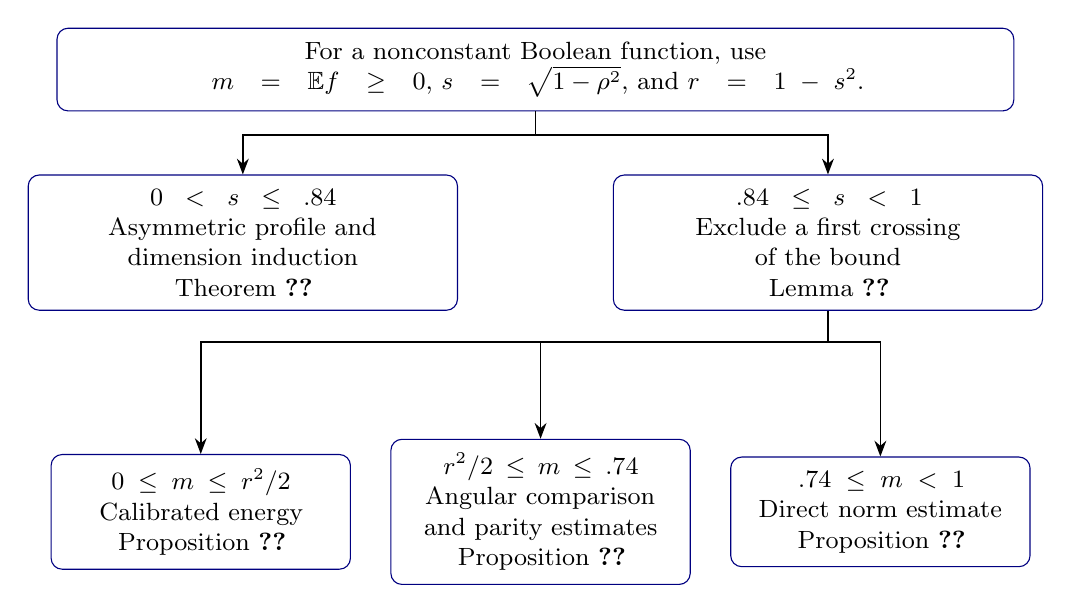
\begin{tikzpicture}[
  box/.style={draw=blue!50!black,rounded corners,align=center,
              inner sep=5pt,font=\small},
  flow/.style={-{Stealth[length=2mm]},semithick},node distance=8mm]
\node[box,text width=11.8cm] (target)
 {For a nonconstant Boolean function, use\\
 $m=\E f\ge0$, $s=\sqrt{1-\rho^2}$, and $r=1-s^2$.};
\node[box,text width=5.1cm,below left=8mm and -5.1cm of target] (ind)
 {$0<s\le .84$\\Asymmetric profile and dimension induction\\
  Theorem~\ref{thm:induction}};
\node[box,text width=5.1cm,below right=8mm and -5.1cm of target] (cont)
 {$.84\le s<1$\\Exclude a first crossing\\of the bound\\
  Lemma~\ref{lem:crossing}};
\draw[flow] (target.south) -- ++(0,-3mm) -| (ind.north);
\draw[flow] (target.south) -- ++(0,-3mm) -| (cont.north);
\node[box,text width=3.45cm,below=23mm of target.south,xshift=-4.25cm,yshift=-2.05cm] (central)
 {$0\le m\le r^2/2$\\Calibrated energy\\Proposition~\ref{prop:central}};
\node[box,text width=3.45cm,right=5mm of central] (mid)
 {$r^2/2\le m\le .74$\\Angular comparison\\and parity estimates\\Proposition~\ref{prop:intermediate}};
\node[box,text width=3.45cm,right=5mm of mid] (large)
 {$.74\le m<1$\\Direct norm estimate\\Proposition~\ref{prop:large-bias}};
\draw[flow] (cont.south) -- ++(0,-4mm) -| (central.north);
\draw[flow] (cont.south) -- ++(0,-4mm) -| (mid.north);
\draw[flow] (cont.south) -- ++(0,-4mm) -| (large.north);
\end{tikzpicture}
\caption{The proof covers all bias and noise parameters. The initial
induction range supplies the starting point for continuation; the three
lower boxes cover every possible nonnegative bias at a proposed crossing.
The large-bias estimate proves the target directly. Endpoints and negative
means are handled by continuity and symmetry.}
\label{fig:proof-regions}
\end{figure}


\paragraph{Organization.}
Section~\ref{sec:preliminaries} fixes the cube conventions.
Section~\ref{sec:induction} proves the dimension-induction range.
Section~\ref{sec:continuation} reduces the rest to excluding an energy crossing.
Sections~\ref{sec:central}, \ref{sec:intermediate}, and \ref{sec:large-bias}
treat the three bias regimes and complete the proof.
Appendix~\ref{app:arithmetic} records the exact-arithmetic conventions;
Appendix~\ref{app:scalar} proves the scalar estimates needed for the induction.

\section{Cube conventions and elementary reductions}\label{sec:preliminaries}
All averages and inner products below use the uniform measure on the relevant cube. For a real function \(u\) on \(\{-1,1\}^n\), write
\[
\chi_S(x)=\prod_{i\in S}x_i,\qquad
\widehat u(S)=\E[u\chi_S],\qquad
u=\sum_{S\subseteq[n]}\widehat u(S)\chi_S.
\]
The functions \(\chi_S\) form an orthonormal basis: independence makes
\(\E\chi_S\chi_T\) equal to \(1\) if \(S=T\) and to \(0\) otherwise.
Consequently,
\[
\Var(u)=\sum_{S\ne\varnothing}\widehat u(S)^2.
\]
For later use set \(W_k(u)=\sum_{|S|=k}\widehat u(S)^2\).

Let \(\E_i\) average only coordinate \(i\), and define
\[
D_i=I-\E_i,\qquad \mathcal N=\sum_{i=1}^n D_i.
\]
Thus \(D_i u(x)=(u(x)-u(x^{(i)}))/2\), where \(x^{(i)}\) reverses coordinate \(i\).
The projections \(D_i\) are self-adjoint and satisfy
\begin{equation}\label{eq:dirichlet}
\E[u\mathcal N v]
=\sum_i\E[D_i u\,D_i v]
=\sum_S |S|\,\widehat u(S)\widehat v(S).
\end{equation}
Independence in the noise definition gives
\(T_\rho\chi_S=\rho^{|S|}\chi_S\). Hence, for \(\tau\ge0\),
\(T_{e^{-\tau}}=e^{-\tau\mathcal N}\).
These elementary facts are also standard in the analysis of Boolean functions~\cite{ODonnell14}; their normalizations are specified here to fix every factor of two.

We first remove the endpoints and symmetries.
The identity
\[
T_{-\rho}f(x)=T_\rho f(-x)
\]
shows that it suffices to consider \(\rho\ge0\). At \(\rho=0\), the left side of Equation~\eqref{eq:main} is zero. At \(\rho=1\), it equals \(H(m)\le1\). For a constant \(f\), it is again zero.
For \(0<\rho<1\) and nonconstant \(f\), every input has positive noise probability, so
\[
-1<T_\rho f(x)<1\qquad\text{for every }x.
\]
All differentiations involving \(H\) below are therefore legitimate. Finally,
replacing \(f\) by \(-f\) preserves both sides of Equation~\eqref{eq:main} and reverses \(m\).


\section{Dimension induction}
\label{sec:induction}

We first prove the desired inequality in the range reached by dimension
induction.  Every decimal in this section denotes an exact rational number.

\begin{theorem}\label{thm:induction}
Let $f:\{-1,1\}^n\to\{-1,1\}$, let $m=\E f$, and let
$0<\rho<1$.  If $s=\sqrt{1-\rho^2}\le .84$, then
\[
  \E H(T_\rho f)\ge H(m)-1+s.
\]
\end{theorem}

We strengthen the desired bound to an inequality for a nonsymmetric
function of the noisy output.  Averaging this inequality with its
reflected version will recover $H$.
The induction uses an asymmetric function $G$ and a polynomial profile $B$.
The scalar inequalities that support it are stated in Lemma~\ref{lem:scalar}
and proved by the finite arithmetic certificates in Appendix~\ref{app:scalar}.
We first establish the two reductions that explain their domains.

\subsection{Compression and a small coordinate}

The following sorting argument is the concave-profile form of the
compression principle of Anantharam, Bogdanov, Chakrabarti, Jayram, and
Nair~\cite[Proposition~2]{ABCJN}. We include the short proof to specify
its direction for $H$.
We order the cube coordinatewise using $-1<1$. A function is
\emph{increasing} if it is nondecreasing in each coordinate.

\begin{lemma}[Compression]\label{ind:lem:compression}
For every Boolean function $f$ there is an increasing Boolean function
$\widetilde f$ with the same mean such that
\[
  \E H(T_\rho\widetilde f)\le \E H(T_\rho f).
\]
\end{lemma}

\begin{proof}
Fix a coordinate, and write $f_-,f_+$ for its two sections.  Replace them
pointwise by $\min(f_-,f_+),\max(f_-,f_+)$, respectively.  Let $T$ denote
noise in the remaining coordinates and put
\[
 a=T\bigl((f_-+f_+)/2\bigr),\qquad
 c=T\bigl((f_+-f_-)/2\bigr).
\]
Sorting preserves $a$ and replaces $c$ by
\[
 c'=T\bigl(|f_+-f_-|/2\bigr)\ge |c|,
\]
since $T$ has a nonnegative kernel.  The two fully noised values are
$a\pm\rho c$ before sorting and $a\pm\rho c'$ afterwards.  For fixed $a$,
the function $u\mapsto H(a+u)+H(a-u)$ is even and concave on its domain,
and hence nonincreasing for $u\ge0$.  Thus sorting weakly decreases the
pair average of $H$.  It preserves the mean.

Perform this operation once in each coordinate.  If the function is
already increasing in a different coordinate, both its sections are
increasing in that coordinate; their pointwise minimum and maximum remain
increasing. The resulting function is therefore increasing in every
coordinate.
\end{proof}

Call a coordinate \emph{active} if the function depends on it.  Inactive
coordinates may be omitted from all expectations below.  Define
\begin{equation}\label{ind:eq:b}
 b(m)=\min\left\{\frac38,\frac9{16}-\frac{|m|}{2},1-|m|\right\},
 \qquad -1\le m\le1.
\end{equation}

\begin{lemma}[Choice of a coordinate]\label{ind:lem:coordinate}
If an increasing Boolean function of mean $m$ has at least four active
coordinates, one of them has first-level coefficient
\[
 0<x=\E[f(X)X_i]\le b(m).
\]
The two sections in this coordinate have means $m-x$ and $m+x$.
\end{lemma}

\begin{proof}
For an increasing Boolean function, the coefficient of coordinate $i$ is
\[
 x_i=\E\bigl[(f_+-f_-)/2\bigr].
\]
The integrand takes values in $\{0,1\}$, so $x_i>0$ precisely when the
coordinate is active.  Choose a coordinate with the least active
coefficient $x$.  For any four distinct active coordinates,
\[
 x\le\frac{x_{i_1}+x_{i_2}+x_{i_3}+x_{i_4}}4
   =\E[f(X)Z],\qquad
 Z=\frac{X_{i_1}+X_{i_2}+X_{i_3}+X_{i_4}}4.
\]
The distribution of $Z$, in decreasing order, is
\[
\begin{array}{c|rrrrr}
z&1&1/2&0&-1/2&-1\\ \hline
\Pr(Z=z)&1/16&4/16&6/16&4/16&1/16.
\end{array}
\]
At fixed mean $m$, the largest possible $\E[fZ]$ is obtained by placing
the positive values of $f$ at the largest values of $Z$, allowing a
fraction of the threshold level.  Indeed, transfer of positive mass from
a smaller value of $Z$ to a larger one can only increase the objective;
allowing fractional values is a relaxation and therefore gives an upper
bound for Boolean $f$.  Since $\E Z=0$ and the law of $Z$ is symmetric,
this maximum is twice the integral over its top fraction
$q=(1-|m|)/2$.  For $q\in[0,1/2]$ that quantity is
\[
 \begin{cases}
 2q,&0\le q\le1/16,\\
 q+1/16,&1/16\le q\le5/16,\\
 3/8,&5/16\le q\le1/2.
 \end{cases}
\]
These are exactly the three pieces of $b(m)$.  Finally, the section
means have average $m$ and half-difference $x$, proving the last claim.
\end{proof}

\subsection{The scalar interface}

For the fixed value of $s$, use one row of
Table~\ref{ind:tab:parameters} whose interval contains $s$.  The profile
polynomials use a finer subdivision of these same intervals, specified
in Appendix~\ref{app:scalar}.  At a shared endpoint, choose the parameters
and the profile consistently from one adjoining interval.  Put
$\delta=(1-\rho)/2$, so that $4\delta(1-\delta)=s^2$; the auxiliary
bounds in the table satisfy $r_0^2\le\delta\le r_1^2$.

\begin{table}[htbp]
\centering
\small
\setlength{\tabcolsep}{3.5pt}
\begin{tabular}{rrrrrrrrrrr}
\toprule
$i$ & $s_{\rm lo}$ & $s_{\rm hi}$ & $r_0$ & $r_1$ & $L$ & $U$ & $V$
    & $\alpha$ & $\Lambda$ & $\mu$\\
\midrule
0 & 0   & 70  & 0   & 36  & 940 & $-440$ & 300 & 960 & 1000 & 956\\
1 & 70  & 160 & 35  & 81  & 940 & $-440$ & 300 & 930 & 1050 & 953\\
2 & 160 & 300 & 80  & 152 & 886 & $-398$ & 250 & 860 & 1150 & 985\\
3 & 300 & 490 & 151 & 254 & 842 & $-335$ & 180 & 770 & 1150 & 1024\\
4 & 490 & 630 & 253 & 335 & 842 & $-335$ & 180 & 690 & 1150 & 1058\\
5 & 630 & 750 & 334 & 412 & 842 & $-335$ & 180 & 632 & 1160 & 1087\\
6 & 750 & 840 & 411 & 479 & 842 & $-335$ & 180 & 583 & 1160 & 1111\\
\bottomrule
\end{tabular}
\caption{Induction parameters.  Every displayed entry except $i$ is
$1000$ times the corresponding parameter.}
\label{ind:tab:parameters}
\end{table}

Define
\begin{equation}\label{ind:eq:G}
 \begin{split}
 \lambda(h)&=L+Uh+Vh^2,\\
 G(p)&=H(2p-1)\left(1+
 \frac{2p-1}{1+H(2p-1)\lambda(H(2p-1))}\right),\qquad 0\le p\le1.
 \end{split}
\end{equation}
All rows have $U<0$, $V\ge0$, and $L+U\ge .488$.  Thus
$\lambda(h)\ge L+U>0$ for $0\le h\le1$, and $G$ is nonnegative,
with $G(0)=G(1)=0$.  Its defining asymmetry cancels under reflection:
\begin{equation}\label{ind:eq:G-reflection}
 G(p)+G(1-p)=2H(2p-1).
\end{equation}

The profiles in the next lemma are explicit polynomials of the form
\begin{equation}\label{ind:eq:profile-def}
 B(m)=(1-m^2)P(m),\qquad
 P(m)=1+10^{-8}\sum_{j\ge1}c_j\bigl(T_j(m)-T_j(0)\bigr),
\end{equation}
where only finitely many $c_j$ are nonzero, and
$T_0(u)=1$, $T_1(u)=u$, $T_{j+1}(u)=2uT_j(u)-T_{j-1}(u)$.
The integer coefficients and their arithmetic verification are given in
Appendix~\ref{app:scalar}.

With these functions, the estimate we will propagate is
\[
 \E G\bigl((1+T_\rho f)/2\bigr)\ge sB(m)
 \qquad(m=\E f)
\]
for every increasing Boolean function $f$.
Its dual $f^*(x)=-f(-x)$ is increasing and has mean $-m$.
Noise commutes with input reversal, so averaging the proposed estimates
for $f$ and $f^*$ and using Equation~\eqref{ind:eq:G-reflection} would give
\[
 \E H(T_\rho f)\ge\frac{s}{2}\bigl(B(m)+B(-m)\bigr).
\]
Thus we need a profile whose reflected average reaches $H(m)-1+s$,
and an estimate for $G$ that passes from two sections to their parent.
The next lemma supplies the two-point gap used in this passage, the
reflected comparison, the condition that closes induction on the
small-coordinate domain, and the initial cases.

\begin{lemma}[Scalar inequalities]\label{lem:scalar}
For every $0<s\le .84$, choose the parameters and the polynomial $B$
as above.  Then $B\ge0$ on $[-1,1]$, $B(0)=1$, $B(\pm1)=0$, and
the following four assertions hold.
\begin{enumerate}
\item For $0\le p_0\le p_1\le1$, write $z=p_1-p_0$ and
$p_u=p_0+uz$, and set
\[
 D=\frac{G(p_\delta)+G(p_{1-\delta})-G(p_0)-G(p_1)}2,
 \qquad S=\alpha G(p_1)+(1-\alpha)G(p_0).
\]
Then $D\ge0$ and
\begin{equation}\label{ind:eq:pair}
 D(S+\Lambda D)\ge
 \mu s^2\left(z-\frac{G(p_1)-G(p_0)}{4L}\right)^2.
\end{equation}
\item For every $m\in[-1,1]$,
\begin{equation}\label{ind:eq:reflection-profile}
 \frac{s}{2}\bigl(B(m)+B(-m)\bigr)\ge H(m)-1+s.
\end{equation}
\item For $m\in[-1,1]$ and $0<x\le b(m)$, put
\[
 B_\pm=B(m\pm x),\qquad
 C=\frac{B_+-B_-}{2x},\qquad
 A=\frac{2B(m)-B_+-B_-}{2x^2}.
\]
Then
\begin{equation}\label{ind:eq:profile}
 A\bigl[B(m)+(2\alpha-1)xC+(\Lambda-1)x^2A\bigr]
 \le \mu\left(1-\frac{s}{2L}C\right)^2.
\end{equation}
\item Every increasing Boolean function depending on at most three
coordinates satisfies
\begin{equation}\label{ind:eq:base}
 \E G\bigl((1+T_\rho f)/2\bigr)\ge sB(\E f).
\end{equation}
\end{enumerate}
\end{lemma}

The four assertions of Lemma~\ref{lem:scalar}, including the entire
three-coordinate base case, are proved in Appendix~\ref{app:scalar}.
We now show how the pair bound and profile comparison propagate the
asymmetric estimate from three active coordinates to arbitrary dimension.

\subsection{Averaging and dimension induction}

\begin{proposition}\label{ind:prop:asymmetric}
For the fixed $s$, parameters, and profile above, every increasing
Boolean function satisfies
\begin{equation}\label{ind:eq:all-dimensions}
 \E G\bigl((1+T_\rho f)/2\bigr)\ge sB(\E f).
\end{equation}
\end{proposition}

\begin{proof}
Induct on the number of active coordinates.  Lemma~\ref{lem:scalar}(4)
provides the cases with at most three.  Otherwise choose the coordinate
in Lemma~\ref{ind:lem:coordinate}, and denote its increasing sections by
$f_-$ and $f_+$, with means $m-x$ and $m+x$.  On the smaller cube let
\[
 p_0=\frac{1+T_\rho f_-}{2},\qquad
 p_1=\frac{1+T_\rho f_+}{2}.
\]
In these expressions, $T_\rho$ acts only on the remaining coordinates.  Positivity of its kernel gives $p_0\le p_1$, and
$\E(p_1-p_0)=x$.  At the two values of the chosen coordinate the parent
noise probabilities are $p_\delta$ and $p_{1-\delta}$.

Apply Equation~\eqref{ind:eq:pair} pointwise, allowing $p_0=p_1$, in
which case both $D$ and the expression on the right vanish.  Set
\[
 y=\frac{\E G(p_1)}s,\qquad t=\frac{\E G(p_0)}s,\qquad
 e=\frac{\E D}s,\qquad k=\frac{s}{2L},\qquad
 Q=\alpha y+(1-\alpha)t.
\]
All of $y,t,e,Q$ are nonnegative.  To average the pair inequality, write
$w=p_1-p_0-(G(p_1)-G(p_0))/(4L)$.  Cauchy--Schwarz yields
\[
 \begin{split}
 (\E D)\,\E(S+\Lambda D)
 &\ge\left(\E\sqrt{D(S+\Lambda D)}\right)^2\\
 &\ge\mu s^2(\E|w|)^2
 \ge\mu s^2(\E w)^2.
 \end{split}
\]
No fixed sign of $w$ is required.  Since
$\E w=x-k(y-t)/2$, division by $s^2$ gives
\begin{equation}\label{ind:eq:averaged-pair}
 e(Q+\Lambda e)\ge\mu\left[x-\frac{k}{2}(y-t)\right]^2.
\end{equation}
The parent expectation divided by $s$ equals $(y+t)/2+e$.  Solving
Equation~\eqref{ind:eq:averaged-pair} for the nonnegative variable $e$
therefore gives the lower bound
\begin{equation}\label{ind:eq:R}
 R_x(y,t)=\frac{y+t}{2}+
 \frac{\sqrt{Q^2+4\Lambda\mu v^2}-Q}{2\Lambda},
 \qquad v=x-\frac{k}{2}(y-t).
\end{equation}

We next justify substitution of the induction bounds into this root.
Put $\Delta=\sqrt{Q^2+4\Lambda\mu v^2}$.  For $y,t>0$,
\[
 \begin{split}
 \partial_yR_x
 &=\frac12-\frac{\alpha}{2\Lambda}
    +\frac{\alpha Q-2\Lambda\mu kv}{2\Lambda\Delta},\\
 \partial_tR_x
 &=\frac12-\frac{1-\alpha}{2\Lambda}
    +\frac{(1-\alpha)Q+2\Lambda\mu kv}{2\Lambda\Delta}.
 \end{split}
\]
Using $Q\ge0$ and
$|v|/\Delta\le1/(2\sqrt{\Lambda\mu})$, each derivative is at least
\begin{equation}\label{ind:eq:root-derivative}
 \frac12\left(1-\frac{\max(\alpha,1-\alpha)}{\Lambda}
              -k\sqrt{\frac\mu\Lambda}\right)>0.
\end{equation}
For completeness, the strict sign follows by rational arithmetic from
Table~\ref{ind:tab:parameters}.  If
$a=1-\max(\alpha,1-\alpha)/\Lambda$, every row has $a>0$ and
\[
 a^2-\left(\frac{s_{\rm hi}}{2L}\right)^2\frac\mu\Lambda
 \ge\frac{12133}{44180000}>0.
\]
Since $s\le s_{\rm hi}$, this proves the sign in
Equation~\eqref{ind:eq:root-derivative}.  Continuity extends
coordinatewise monotonicity of $R_x$ to the whole nonnegative quadrant.

Each section has fewer active coordinates, so the induction hypothesis
implies $y\ge B_+$ and $t\ge B_-$.  We have consequently obtained the
lower bound $R_x(B_+,B_-)$ for the normalized parent expectation.
In the notation of Lemma~\ref{lem:scalar}(3), at these arguments
\[
 \frac{B_++B_-}{2}=B(m)-x^2A,\qquad
 Q=B(m)-x^2A+(2\alpha-1)xC,\qquad
 v=x(1-kC).
\]
If $A\le0$, the first of these terms is already at least $B(m)$,
and the root correction in Equation~\eqref{ind:eq:R} is nonnegative.
Suppose $A>0$.  The correction is the nonnegative solution $u$ of
$u(Q+\Lambda u)=\mu x^2(1-kC)^2$.  Because $Q\ge0$ and $\Lambda>0$,
the left side is increasing for $u\ge0$.  Equation~\eqref{ind:eq:profile},
multiplied by $x^2$, states that
\[
 \begin{split}
 (x^2A)(Q+\Lambda x^2A)
 &=x^2A\bigl[B(m)+(2\alpha-1)xC+(\Lambda-1)x^2A\bigr]\\
 &\le\mu x^2(1-kC)^2.
 \end{split}
\]
Thus the correction is at least $x^2A$, and again
$R_x(B_+,B_-)\ge B(m)$.  This completes the induction.
\end{proof}

\begin{proof}[Proof of Theorem~\ref{thm:induction}]
By Lemma~\ref{ind:lem:compression}, it suffices to consider increasing
$f$.  Its dual $f^*(x)=-f(-x)$ is also increasing and has mean $-m$.
Noise commutes with input reversal, so
$T_\rho f^*(x)=-T_\rho f(-x)$.  Apply
Proposition~\ref{ind:prop:asymmetric} to $f$ and $f^*$, average the two
inequalities, and change variables $x\mapsto-x$ in the second
expectation.  Equation~\eqref{ind:eq:G-reflection} gives
\[
 \E H(T_\rho f)
 \ge\frac{s}{2}\bigl(B(m)+B(-m)\bigr)
 \ge H(m)-1+s,
\]
where the last inequality is Equation~\eqref{ind:eq:reflection-profile}.
\end{proof}

\section{A continuation criterion}\label{sec:continuation}
The notation in this section and the next three is independent of the induction parameters.
Fix a nonconstant Boolean \(f\), use output-sign symmetry to take \(m=\E f\ge0\), and put
\begin{equation}\label{eq:continuation-notation}
\begin{gathered}
s=\sqrt{1-\rho^2},\qquad r=\rho^2=1-s^2,\qquad d=T_\rho f,\\
h=H(m),\qquad b=\E H(d),\qquad v=1-s,\qquad K=\frac rs.
\end{gathered}
\end{equation}
We work with \(.84\le s<1\), so \(0<r\le .2944\).

Define
\begin{equation}\label{eq:energy-definition}
\mathcal E(d)=\E\sum_i D_i d\,D_i\!\left(\frac{d}{H(d)}\right).
\end{equation}
For the parameter \(\tau=-\log\rho\), one has
\(\partial_\tau d=-\mathcal N d\). Since \(H'(z)=-z/H(z)\),
Equation~\eqref{eq:dirichlet} yields
\begin{equation}\label{eq:energy-derivative}
\frac{db}{d\tau}=\mathcal E(d),
\qquad
\frac{ds}{d\tau}=\frac rs=K.
\end{equation}

This identity is the Hellinger edge derivative of
Chen, Gohari, and Nair~\cite[Section~III, Lemma~6]{HellingerDifferential}
in our generator normalization: their parameter has $\rho=e^{-2t}$,
so $\tau=2t$ here.

\begin{lemma}[Crossing criterion]\label{lem:crossing}
Suppose Equation~\eqref{eq:main} is known for \(s\le .84\).
If it fails for some \(s>.84\), then for the same function there is a parameter
\(.84\le s<1\) for which
\begin{equation}\label{eq:crossing}
b=h-1+s,\qquad \mathcal E(d)\le K.
\end{equation}
It is enough to exclude Equation~\eqref{eq:crossing} for functions other than signed coordinates.
\end{lemma}
\begin{proof}
The desired inequality is \(b-h+1-s\ge0\). If this expression is negative at some finite semigroup time, take the left endpoint \(\tau_0\) of the connected component of strict negativity containing that time, restricted to times after \(s=.84\).
Continuity gives equality at \(\tau_0\).
The right difference quotients there are nonpositive, so differentiability and Equation~\eqref{eq:energy-derivative} give the energy inequality in Equation~\eqref{eq:crossing}.
For \(f=\pm x_i\), one has \(m=0\), \(d=\pm\rho x_i\), and \(b=s\), so the desired inequality is an identity for every parameter.
\end{proof}

The following change of variable will be used in the two smaller bias regimes:
\begin{equation}\label{eq:F-definition}
F(x)=\int_0^x(1-z^2)^{-3/4}\,dz,\qquad g=F(d).
\end{equation}
The function \(F\) is odd, increasing, and has finite limits at \(\pm1\).

\begin{lemma}[Basic energy comparison]\label{lem:basic-energy}
With the preceding notation,
\begin{equation}\label{eq:basic-energy}
\mathcal E(d)\ge\sum_i\E(D_i g)^2\ge\Var(g).
\end{equation}
\end{lemma}
\begin{proof}
For the two values \(z_-\le z_+\) of \(d\) on an edge, the edge contributions have the respective forms
\[
\frac14(z_+-z_-)\left(\frac{z_+}{H(z_+)}-\frac{z_-}{H(z_-)}\right),
\qquad
\frac14(F(z_+)-F(z_-))^2.
\]
The derivative of \(x/H(x)\) is \(H(x)^{-3}=(F'(x))^2\), so Cauchy--Schwarz on \([z_-,z_+]\) compares these in the required direction. The case \(z_-=z_+\) follows by continuity. Summing over edges proves the first inequality.
The second follows from Equation~\eqref{eq:dirichlet}, since every nonconstant Fourier degree is at least one.
\end{proof}

The two smaller bias ranges will combine these energy comparisons with
upper bounds on the variance of $d$ and its odd part.  Booleanity supplies
the following bounds.

\begin{lemma}[Boolean spectral bounds]\label{lem:fourier-bounds}
Set
\[
p=\frac{1-m}{2},\qquad
w=\min\left\{2p,\;4\sqrt{\frac32}\,p^{3/2}\right\}.
\]
Then
\begin{align}
W_1(f)&\le w,\label{eq:first-level-bound}\\
\Var(d)&\le r[(1-r)w+rh^2].\label{eq:variance-bound}
\end{align}
If \(d_{\rm o}(x)=(d(x)-d(-x))/2\) is the odd part of \(d\), then
\begin{equation}\label{eq:odd-variance-bound}
\E d_{\rm o}^2\le r[(1-r^2)w+r^2h^2].
\end{equation}
\end{lemma}
\begin{proof}
Write \(L_+=\max(L,0)\) and \(L_-=\max(-L,0)\).
For a homogeneous linear form \(L=\sum_i a_i x_i\) with \(\E L^2=1\), symmetry gives
\(\E L_+^2=1/2\), while expansion gives
\[
\E L^4=3\left(\sum_i a_i^2\right)^2-2\sum_i a_i^4\le3,
\qquad \E L_+^4\le3/2.
\]
Let \(A=\{f=-1\}\), of measure \(p\).
Since \(\E L=0\),
\(\E fL=-2\E[1_A L]\).
The absolute value of the last integral is at most the larger of
\(\E[1_A L_+]\) and \(\E[1_A L_-]\).
Hölder's inequality therefore gives
\[
|\E fL|\le
2\min\left\{\sqrt{p/2},\;(3/2)^{1/4}p^{3/4}\right\}.
\]
Maximizing over \(L\) and squaring proves Equation~\eqref{eq:first-level-bound}.
Parseval and Booleanity give
\(\sum_{k\ge1}W_k(f)=1-m^2=h^2\).
Thus
\[
\Var(d)=\sum_{k\ge1}r^kW_k(f)
\le rW_1(f)+r^2(h^2-W_1(f)),
\]
which proves Equation~\eqref{eq:variance-bound}.
The odd part retains only odd degrees. Every retained degree above one is at least three, so
\[
\E d_{\rm o}^2
\le rW_1(f)+r^3(h^2-W_1(f)),
\]
proving Equation~\eqref{eq:odd-variance-bound}.
\end{proof}

At a hypothetical crossing, the fixed mean lies either in the central band
\(0\le m\le r^2/2\), in the intermediate band \(r^2/2\le m\le .74\), or in the large-bias band \(.74\le m<1\).
The next sections exclude the crossing in the first two bands and prove the target directly in the third.

\section{The central band}\label{sec:central}

We retain the notation of Section~\ref{sec:continuation}.  In the band
containing the signed coordinates, we sharpen the basic energy comparison
to preserve their exact edge cost.  The resulting bound will force any
function satisfying the crossing conditions to be a signed coordinate.

\begin{proposition}\label{prop:central}
Let $f$ be a nonconstant Boolean function, let $0<\rho<1$, and suppose that
$s\ge .84$ and $0\le m\le r^2/2$.  If
\begin{equation}\label{cen:crossing}
 b=h-1+s,\qquad \mathcal E(d)\le K=\frac rs,
\end{equation}
then $f$ is a signed coordinate.
\end{proposition}

Throughout the proof all terminating decimals denote exact rational
numbers.  Under \eqref{cen:crossing}, set
\begin{equation}\label{cen:calibration}
 y=\sqrt b,\qquad x_0=\sqrt{1-b^2},\qquad
 \alpha=\frac{F(x_0)}{x_0},\qquad M=F(x_0)^2.
\end{equation}
The symbol $\alpha$ is local to this section.  Write $R_0=.2944$.  Since
$0<r\le R_0$ and $m\le R_0^2/2$, the exact comparison
$(.999)^2<1-R_0^4/4$ gives
\begin{equation}\label{cen:domain}
 \begin{gathered}
 h>.999,\qquad .839<b\le s<1,\qquad y>.91595>.915,\\
 0\le s-b=\frac{m^2}{1+h}<.001,\qquad M\ge x_0^2\ge r>0.
 \end{gathered}
\end{equation}
Here $F(x)\ge x$ for $x\ge0$, and $(.91595)^2<.839$.
The symmetric pair of values $\pm x_0$ has $H(x_0)=b$, so its
$H$-average equals that of $d$ and its transformed squared amplitude is $M$.
Its edge energy is $x_0^2/b$.  When $m=0$, the crossing identity gives
$b=s$ and $x_0=\rho$, recovering a noised coordinate.

\subsection{The calibrated edge cost}

For $0\le v<F(1)^2$, define
\begin{equation}\label{cen:phi}
 \Phi(v)=\frac{x^2}{H(x)}-v,
 \qquad x=F^{-1}(\sqrt v),\qquad
 j(v)=\begin{cases}\Phi(v)/v,&v>0,\\0,&v=0.\end{cases}
\end{equation}
The endpoint value $F(1)$ is finite, since the integrand defining $F$ has
an integrable singularity of order $3/4$ at $1$.

\Needspace{6\baselineskip}
\begin{lemma}[Calibrated edge comparison]\label{cen:edge}
For every coordinate edge,
\begin{equation}\label{cen:edge-bound}
 D_i d\,D_i\!\left(\frac d{H(d)}\right)
 \ge (D_i g)^2+\Phi\bigl((D_i g)^2\bigr).
\end{equation}
The functions $j$ and $\Phi$ are nonnegative, increasing, and convex.
Furthermore, $\Phi'(v)/v$ is increasing for $v>0$.
\end{lemma}

\begin{proof}
Put $G=F(x)$ and $\ell(G)=\log F'(x)$.  Direct differentiation gives
\begin{equation}\label{cen:ell}
 \ell'(G)=\frac{3x}{2\sqrt{H(x)}},\qquad
 \ell''(G)=\frac34\left(H(x)+\frac1{H(x)}\right),\qquad
 \ell'''(G)=\frac{3x^3}{4H(x)^{3/2}}.
\end{equation}
Thus $\ell$ is even and convex, and $\ell''$ is increasing on the
nonnegative half of its domain.

Consider an edge with distinct $g$-values $G_-<G_+$, and let
$I=[G_-,G_+]$.  Changing variables from $x$ to $G$ in the two differences
shows that the ratio of its energy to $(D_i g)^2$ is
\[
 \left(\frac1{|I|}\int_I e^{\ell(G)}\,dG\right)
 \left(\frac1{|I|}\int_I e^{-\ell(G)}\,dG\right)
 =\E\cosh\bigl(\ell(U)-\ell(V)\bigr),
\]
where $U,V$ are independent uniform points of $I$.  For a fixed separation
$\delta=|U-V|$, the midpoint is uniform on the interval of length
$|I|-\delta$ with the same center as $I$.  The function
\[
 A_\delta(c)=\ell(c+\delta/2)-\ell(c-\delta/2)
\]
is odd, and is increasing because
$A_\delta'(c)=\ell'(c+\delta/2)-\ell'(c-\delta/2)\ge0$.
Consequently $\cosh A_\delta(c)$ is even and increasing in $|c|$.
The integral of any such function over an interval of fixed length is
minimized by centering that interval at zero: for positive center $c$,
the derivative of the integral is the value at the right endpoint minus
the value at the left endpoint, which is nonnegative.  The domain of $\ell$ is the symmetric interval $(-F(1),F(1))$.
Moving the center of $I$ toward zero while keeping its length fixed
keeps $I$, and hence every conditional midpoint interval, in this domain.
Applying the preceding fixed-length integral comparison conditionally
on $\delta$ proves that the displayed product of averages is minimized
when $I$ is centered at zero.

If that centered interval has endpoints $\pm a$, its corresponding
$d$-values are $\pm x$, where $F(x)=a$.  Its energy is exactly
$x^2/H(x)=a^2+\Phi(a^2)$.  Since $a^2=(D_i g)^2$, this proves
\eqref{cen:edge-bound}.  A zero difference gives the same statement
directly.

The symmetric-interval computation also gives, for $v>0$,
\begin{equation}\label{cen:j-average}
 j(v)=\frac14\int_{-1}^1\int_{-1}^1
 \left[\cosh\bigl(\ell(\sqrt v\,a)-\ell(\sqrt v\,c)\bigr)-1\right]
 \,da\,dc.
\end{equation}
To prove convexity of the integrand in $v$, use evenness of $\ell$ and
$\cosh$ to replace $(a,c)$ by numbers $A\ge C\ge0$.
For $B(v)=\ell(A\sqrt v)-\ell(C\sqrt v)$, differentiation gives
\[
 B'(v)=\frac{z_A\ell'(z_A)-z_C\ell'(z_C)}{2v},\qquad
 B''(v)=\frac{Q(z_A)-Q(z_C)}{4v^2},
 \quad z_A=A\sqrt v,\ z_C=C\sqrt v,
\]
where $Q(z)=z(z\ell''(z)-\ell'(z))$.
The function $z\ell'(z)$ is increasing on $z\ge0$, and
\[
 Q'(z)=z\ell''(z)-\ell'(z)+z^2\ell'''(z)\ge0.
\]
Indeed, $\ell'(0)=0$ and increasing $\ell''$ imply
$\ell'(z)\le z\ell''(z)$, and \eqref{cen:ell} gives $\ell'''(z)\ge0$.
Thus $B$ is nonnegative, increasing, and convex.  Its composition with
$\cosh-1$ has the same properties.  Averaging proves these properties
for $j$, including its continuous extension $j(0)=0$.
Now $\Phi(v)=vj(v)$ gives
$\Phi'=j+vj'\ge0$ and $\Phi''=2j'+vj''\ge0$.
Finally, convexity and $j(0)=0$ imply that $j(v)/v$ is increasing, while
$j'$ is increasing.  Therefore
\[
 \frac{\Phi'(v)}v=\frac{j(v)}v+j'(v)
\]
is increasing as claimed.
\end{proof}

Define the slope and energy excess at the calibration by
\begin{equation}\label{cen:pdelta}
 p_*:=\Phi'(M)=\frac{1+b^2}{2\alpha b^{3/2}}-1,\qquad
 \Delta:=M+\Phi(M)-K=(s-b)\left(1+\frac1{bs}\right).
\end{equation}
The first identity follows by differentiating $x^2/H(x)$ with respect
to $F(x)^2$; the second uses
$M+\Phi(M)=(1-b^2)/b$ and $K=(1-s^2)/s$.
In particular, $p_*,\Delta\ge0$.

\begin{lemma}[Calibration bounds]\label{cen:constants}
At a crossing in the central band,
\begin{equation}\label{cen:four-constants}
 \frac{\Phi(M)}M<.0063,\qquad p_*<.019,\qquad
 \frac{p_*}M<.0532,\qquad \frac\Delta M<.008.
\end{equation}
\end{lemma}

\begin{proof}
As $b$ decreases, $M$ increases.  Lemma~\ref{cen:edge} therefore reduces
the first three upper bounds to $b_0=.839$.  Set
$\alpha_0=F(\sqrt{1-b_0^2})/\sqrt{1-b_0^2}$.
At this endpoint the positive binomial series, integrated term by term,
gives
\[
 \alpha_0\ge\sum_{j=0}^{5}
 \frac{(3/4)_j(1-b_0^2)^j}{j!(2j+1)}>a_0:=1.08834,
 \qquad \sqrt{b_0}>y_0:=.91595,
\]
where $(3/4)_0=1$ and $(3/4)_j=(3/4)(7/4)\cdots(3/4+j-1)$.
Using $\Phi(M)/M=1/(b\alpha^2)-1$ and \eqref{cen:pdelta}, exact rational
comparisons give
\begin{align*}
 \frac1{b_0a_0^2}-1&<.006257<.0063,\\
 P_0:=\frac{1+b_0^2}{2a_0b_0y_0}-1&<.018641<.019,\\
 \frac{P_0}{(1-b_0^2)a_0^2}&<.053154<.0532.
\end{align*}
For the last bound, \eqref{cen:domain} and $m^2\le r^4/4$ give
\[
 \frac\Delta M\le
 \frac{r^3}{4(1+h)}\left(1+\frac1{bs}\right)
 <\frac{R_0^3}{4(1.999)}
       \left(1+\frac1{(.839)(.84)}\right)<.007720<.008.
\]
The numerical comparisons above are exact rational inequalities.
The four bounds in \eqref{cen:four-constants} are also verified by the
central-band certificate described in Appendix~\ref{app:arithmetic}.
\end{proof}

\subsection{Reduction to variance and first-level estimates}

Let $a_i$ be
the degree-one Fourier coefficients of $g$, and put
\[
 q=\sum_i a_i^2,\qquad l=\max_i a_i^2,\qquad H_0=\Var g-q.
\]
Thus $H_0$ is the Fourier weight above degree one.  Counting degrees gives
$\sum_i\E(D_i g)^2\ge\Var g+H_0$.
All arguments of $\Phi$ used below belong to its open domain:
since the cube is finite, $G_{\max}:=\max|g|<F(1)$; every half-difference
$|D_i g|$ and coefficient $|a_i|$ is at most $G_{\max}$, while
$M=F(x_0)^2<F(1)^2$ because $b>0$.
In a coordinate attaining $l$, Jensen's inequality and monotonicity of
$\Phi$ give
$\E\Phi((D_i g)^2)\ge\Phi(\E(D_i g)^2)\ge\Phi(l)$.
Lemma~\ref{cen:edge} and the tangent inequality for $\Phi$ at $M$ yield
\begin{align}
 \mathcal E(d)&\ge\Var g+H_0+\Phi(l)\label{cen:spectral-energy}\\
 &\ge K+(1+p_*)(\Var g-M)+(1-p_*)H_0
             -p_*(q-l)+\Delta.\label{cen:tangent-energy}
\end{align}

Here $q-l$ is the degree-one weight outside a largest coordinate.
Put
\begin{equation}\label{cen:V0}
 V_0=\E(g^2-M)^2,\qquad C_0=.034.
\end{equation}
We will prove
\begin{equation}\label{cen:variance-gain}
 \Var g-M\ge C_0V_0-\frac\Delta{1+p_*},
\end{equation}
with strict inequality unless $m=0$ and $g^2=M$ everywhere.
Substituting this estimate into \eqref{cen:tangent-energy} cancels
$\Delta$.  We will then control the remaining negative term by proving
\[
 p_*(q-l)\le(1+p_*)C_0V_0+(1-p_*)H_0.
\]
These two bounds give $\mathcal E(d)>K$ whenever the variance inequality
is strict.  We first prove that inequality, then establish the
first-level comparison and treat the remaining equality case.

\subsection{A variance gain around the calibration}

Define, on $0\le t<1$,
\[
 k(t)=\frac{F(\sqrt{1-t^4})}{\sqrt{1-t^4}},\qquad k(1)=1.
\]
Writing $u=\sqrt{H(d)}$, one has $g=k(u)d$, $k(y)=\alpha$, and
\begin{equation}\label{cen:k-ode}
 k'(t)=-\frac{2(1-t^3k(t))}{1-t^4},\qquad
 g^2-M=-4\int_y^u k(t)\,dt.
\end{equation}
Both identities follow by differentiation; the second also holds at
$u=1$ by continuity.

\begin{lemma}[Bounds for the comparison function]\label{cen:k-bounds}
For $0\le t\le1$,
\begin{equation}\label{cen:k-estimates}
 2-t+\tfrac12(1-t)^2\le k(t)\le2-t+\tfrac34(1-t)^2,
 \qquad
 1\le-k'(t)\le\min\{2,1+\tfrac32(1-t)\}.
\end{equation}
At $t=1$, the derivative is understood as its left limit.
\end{lemma}

\begin{proof}
For $P_c(t)=2-t+c(1-t)^2$, define the differential residual
\[
 E_c(t)=-(1-t^4)P_c'(t)-2(1-t^3P_c(t)).
\]
Expansion yields
\begin{align*}
 \frac{E_{1/2}(t)}{(1-t)^2}&=t(2t^2-2t-1)\le0,\\
 \frac{E_{3/4}(t)}{(1-t)^2}
 &=\tfrac12(2t+1)(3t^2-3t+1)>0.
\end{align*}
The first sign uses $2t^2-2t-1\le-1$; for the second,
$3t^2-3t+1=3(t-1/2)^2+1/4$.
To justify backward comparison despite the singular endpoint, fix
$t<v<1$.  The error $e=k-P_c$ satisfies
$e'-2t^3e/(1-t^4)=E_c/(1-t^4)$, whence
\[
 e(t)=\sqrt{\frac{1-v^4}{1-t^4}}\,e(v)
 -\int_t^v\sqrt{\frac{1-z^4}{1-t^4}}
                   \frac{E_c(z)}{1-z^4}\,dz.
\]
Both $k(v)$ and $P_c(v)$ tend to $1$.  The first term therefore vanishes
as $v\uparrow1$, and the integral converges.  Its sign proves the two
polynomial comparisons in \eqref{cen:k-estimates}.

Substitute these comparisons into \eqref{cen:k-ode}.  The sufficient
numerators for the three derivative inequalities are, respectively,
\begin{align*}
 2(1-t^3P_{3/4})-(1-t^4)
   &=\tfrac12(1-t)^2(-3t^3+6t^2+4t+2),\\
 2(1-t^4)-2(1-t^3P_{1/2})
   &=t^3(t-5)(t-1),\\
 \tfrac{5-3t}{2}(1-t^4)-2(1-t^3P_{1/2})
   &=\tfrac12(1-t)^2(5t^3-3t^2-t+1).
\end{align*}
The first two are nonnegative on $[0,1]$.  For the last cubic, on
$[0,.6]$ use
$5t^3-3t^2+.16=(5t+1)(5t-2)^2/25\ge0$, leaving at least $.24$.
On $[.6,1]$ write the cubic as $t^2(5t-3)+(1-t)\ge0$.
This proves the derivative bounds for $t<1$.  The Taylor expansion
$F(x)/x=1+x^2/4+O(x^4)$ at $x=0$ shows that $k'(1)=-1$.
\end{proof}

To estimate the variance of $g$, separate its mean from the known mean
$\E d=m$ by subtracting $\alpha d$.  Define
\begin{equation}\label{cen:RD}
 R=g-\alpha d,\qquad
 D(u)=g^2-M-R^2+\frac{2\alpha}{y}(u^2-y^2).
\end{equation}
The right side defining $D$ depends only on $u$, because
$R^2=(1-u^4)(k(u)-\alpha)^2$.  The added multiple of $u^2-y^2$
has zero expectation.  Since $\E u^2=b=y^2$, $\E g=\E R+\alpha m$, and
$(\E R)^2\le\E R^2$, one obtains
\begin{equation}\label{cen:variance-rearrange}
 \Var g-M\ge\E\bigl[D-2\alpha m|R|\bigr]-\alpha^2m^2.
\end{equation}

\begin{lemma}[Pointwise remainder bound]\label{cen:pointwise}
Under the central-band crossing hypotheses of Proposition~\ref{prop:central},
for every $0\le u\le1$,
\begin{equation}\label{cen:pointwise-bound}
 D(u)-2\alpha m|R|+.88m^2
 \ge C_0(g^2-M)^2+.20(u^2-y^2)^2.
\end{equation}
The inequality is strict whenever $u\ne y$.
\end{lemma}

\begin{proof}
The integral identity in \eqref{cen:k-ode} gives exactly
\begin{equation}\label{cen:D-integral}
 D(u)=\frac{2\alpha}{y}(u-y)^2
       +4\int_u^y(k(t)-\alpha)\,dt
       -(1-u^4)(k(u)-\alpha)^2.
\end{equation}
Let $L=|u-y|$ and $\lambda=|k(u)-k(y)|$.  Monotonicity of $k$ makes
the integral nonnegative.  A function with slope of magnitude at most
$2$ needs length at least $\lambda/2$ to rise from $0$ to $\lambda$;
the triangle of that base and height is a lower bound for its integral.
Thus
\[
 4\int_u^y(k(t)-\alpha)\,dt\ge\lambda^2.
\]
The lower derivative bound in Lemma~\ref{cen:k-bounds} gives
$\lambda\ge L$, so \eqref{cen:D-integral} implies
\begin{equation}\label{cen:D-lower}
 D(u)\ge\left(\frac{2\alpha}{y}+u^4\right)L^2.
\end{equation}

For explicit estimates, put $a=1-u$, $c=1-y$, and
\begin{align*}
 A_-&=1+c+\tfrac12c^2,& A_+&=1+c+\tfrac34c^2,\\
 B&=1+\tfrac12(a+c)+\tfrac14(a^2+ac+c^2),&
 J&=1+\tfrac34(a+c).
\end{align*}
Lemma~\ref{cen:k-bounds}, and its averages over the interval joining
$u$ and $y$, give
\begin{equation}\label{cen:BJ}
 A_-\le\alpha\le A_+,\qquad
 |g^2-M|\le4BL,\qquad
 |R|\le J L\sqrt{1-u^4}.
\end{equation}
In fact $B$ is the average of the upper quadratic bound for $k$, and
$J$ is the average of the upper linear bound for $-k'$.
Define
\begin{equation}\label{cen:S}
 S(u,y)=2A_-+y\bigl(u^4-16C_0B^2-.20(u+y)^2\bigr).
\end{equation}
By \eqref{cen:D-lower}--\eqref{cen:BJ}, the left side minus the right
side of \eqref{cen:pointwise-bound} is at least
\begin{equation}\label{cen:pointwise-reduction}
 \frac{L^2}{y}S
 -2A_+JmL\sqrt{1-u^4}+.88m^2.
\end{equation}
If $u\le .8$, then $L=y-u>0$.  Since $b\le s$ and $2m\le r^2$,
\[
 2m\le r^2\le(1-b^2)^2=(1-y^4)^2.
\]
Dropping $.88m^2$ and bounding $\sqrt{1-u^4}\le1$ makes
\eqref{cen:pointwise-reduction} at least $LP_1/y$, where
\begin{equation}\label{cen:P1}
 P_1(u,y)=(y-u)S-A_+J(1-y^4)^2y.
\end{equation}
If $u\ge .8$ and $L>0$, the elementary inequality
\[
 2A_+JmL\sqrt{1-u^4}
 \le .88m^2+\frac{(A_+J)^2L^2(1-u^4)}{.88}
\]
makes the same expression at least $L^2P_2/(.88y)$, where
\begin{equation}\label{cen:P2}
 P_2(u,y)=.88S-(A_+J)^2(1-u^4)y.
\end{equation}
It therefore suffices, when $L>0$, to prove the polynomial signs
\begin{equation}\label{cen:polynomial-signs}
 \begin{aligned}
 P_1(u,y)&>0 &&(0\le u\le .8,\ .915\le y\le1),\\
 P_2(u,y)&>0 &&(.8\le u\le1,\ .915\le y\le1).
 \end{aligned}
\end{equation}
Here is a finite rational certificate for these signs, using the Bernstein
coefficient formula of Appendix~\ref{app:arithmetic}. Map each stated
rectangle affinely to $[0,1]^2$, with the $u$ coordinate first.  If the
resulting power coefficients are $c_{ab}$, its Bernstein coefficient of
index $(i,j)$ and order $(N_1,N_2)$ is
\begin{equation}\label{cen:bernstein-formula}
 \beta_{ij}=\sum_{a\le i,\,b\le j}c_{ab}
       \frac{\binom ia}{\binom{N_1}a}
       \frac{\binom jb}{\binom{N_2}b}.
\end{equation}
The orders and row minima are as follows; the final column records
$\lfloor1000\min_j\beta_{ij}\rfloor$ for successive $i$.
\begin{center}
\begin{tabular}{@{}ccl@{}}
\toprule
Polynomial & Order $(N_1,N_2)$ & Scaled row minima \\
\midrule
$P_1$ & $(5,12)$ & $134,353,365,278,214,46$ \\
$P_2$ & $(6,7)$ & $179,364,559,765,983,1214,1457$ \\
\bottomrule
\end{tabular}
\end{center}
Thus every coefficient is strictly positive.  Bernstein basis functions
are nonnegative and sum to one on the unit square, proving
\eqref{cen:polynomial-signs} on the closed rectangles.  The formula and
the explicit polynomials specify all arithmetic in the table; the
executable certificate is \texttt{verification/central\_band.py}.
Appendix~\ref{app:arithmetic} gives the general certificate convention.

The two lower bounds above are therefore strictly positive whenever
$L>0$.
Finally, when $u=y$, all terms in \eqref{cen:pointwise-bound} vanish
except $.88m^2$, which is nonnegative.  This also proves the asserted
strictness.
\end{proof}

\begin{lemma}[Strict variance gain]\label{cen:strict-variance}
Inequality \eqref{cen:variance-gain} holds.  If $m>0$, the stronger bound
\begin{equation}\label{cen:positive-margin}
 \Var g-M>C_0V_0-\frac\Delta{1+p_*}+.016m^2
\end{equation}
holds.  If $m=0$, \eqref{cen:variance-gain} is strict unless $g^2=M$
at every point of the cube.
\end{lemma}

\begin{proof}
Write $T=\E(u^2-y^2)^2=\E(H(d)-b)^2$.
Since $\E d=m$ and $H(d)^2=1-d^2$,
$T=h^2-b^2-\Var d$.  Lemma~\ref{lem:fourier-bounds}, using $w\le1-m$,
therefore gives
\[
 T\ge(1-r^2)h^2-b^2-rs^2(1-m).
\]
The crossing identity implies $sh-b=(1-s)(1-h)\ge0$.
Substituting $b^2\le s^2h^2$ proves
\begin{equation}\label{cen:T-lower}
 T\ge rs^2(m-m^2).
\end{equation}
For $m>0$ this yields
\begin{equation}\label{cen:T-ratio}
 \frac T{m^2}\ge s^2\left(\frac2r-r\right)
 \ge(1-R_0)\left(\frac2{R_0}-R_0\right)>4.5.
\end{equation}
Both positive factors in the middle expression decrease with $r$ on
$0<r\le R_0$, and the final inequality is rational.

We also need to compare the calibration loss with $\alpha^2m^2$.
The upper bound for $k(y)$ gives $\alpha<1.1$ and
\[
 \alpha y\le(1-c)(1+c+\tfrac34c^2)
       =1-\tfrac14c^2-\tfrac34c^3\le1,
 \qquad c=1-y\in[0,.085].
\]
Using \eqref{cen:pdelta} and $s-b=m^2/(1+h)$, for $m>0$ we obtain
\begin{align}
 \frac\Delta{(1+p_*)m^2}
 &=\frac\alpha y\,\frac2{1+h}
       \left(1-\frac{s-b}{s(1+b^2)}\right)\label{cen:delta-cancel}\\
 &>\alpha^2-\frac{(1.1)^2(.001)}{.84}
 >\alpha^2-.004.\notag
\end{align}
In the first factor of \eqref{cen:delta-cancel}, $\alpha/y\ge\alpha^2$;
also $2/(1+h)\ge1$.  The subtracted relative loss is less than
$.001/.84$, by \eqref{cen:domain}, which proves the next line.

Averaging \eqref{cen:pointwise-bound} and applying
\eqref{cen:variance-rearrange} now gives
\[
 \Var g-M\ge C_0V_0+.20T-(\alpha^2+.88)m^2.
\]
For $m>0$, insert \eqref{cen:T-ratio} and \eqref{cen:delta-cancel}.
The remaining strict margin is
$.20(4.5)-.88-.004=.016$, proving \eqref{cen:positive-margin}.
For $m=0$ one has $b=s$ and $\Delta=0$; the same averaged inequality
proves \eqref{cen:variance-gain}.  If any cube point has $u\ne y$,
Lemma~\ref{cen:pointwise} makes the averaged inequality strict.
Since $k>0$ in \eqref{cen:k-ode}, the condition $u=y$ is equivalent to
$g^2=M$, completing the strictness statement.
\end{proof}

\subsection{Concentration of the first Fourier level}

\begin{proof}[Proof of Proposition~\ref{prop:central}]
Recall that $q$ is the total degree-one Fourier weight of $g$, $l$ is
its largest coordinate weight, and $H_0=\Var g-q$ is its weight above
degree one.

The resources available to control $q-l$ follow without losing the
$\Delta$ term.  Namely, \eqref{cen:crossing},
\eqref{cen:spectral-energy}, and \eqref{cen:variance-gain} imply
\begin{equation}\label{cen:resources}
 H_0+C_0V_0\le\Phi(M)-\frac{p_*\Delta}{1+p_*}\le\Phi(M),
 \qquad
 q\ge M-\Phi(M)-\Delta>.985M>0.
\end{equation}
Indeed, substituting the variance gain into the first energy bound gives
\[
 H_0+C_0V_0\le K-M+\frac{\Delta}{1+p_*}-\Phi(l)
 =\Phi(M)-\frac{p_*\Delta}{1+p_*}-\Phi(l).
\]
Since $\Phi(l)\ge0$, this proves the first resource bound. Combining it
with the variance gain once more yields
\[
 q\ge M-\Phi(M)+2C_0V_0+\frac{p_*-1}{1+p_*}\Delta
 \ge M-\Phi(M)-\Delta.
\]
Thus the second inequality retains the full calibration loss;
Lemma~\ref{cen:constants} gives
$1-.0063-.008=.9857>.985$.

Let
\[
 L_1(x)=\sum_i a_i x_i,\qquad P=L_1^2-q,\qquad
 W=\E P^2=2\left(q^2-\sum_i a_i^4\right).
\]
Since $\sum_i a_i^4\le lq$,
\begin{equation}\label{cen:spread}
 q-l\le\frac W{2q}.
\end{equation}
Write $g=\mu+L_1+Z$, with $\mu=\E g$ and $Z$ containing only Fourier
degrees at least two; thus $\E Z^2=H_0$.
The degree-three part of $L_1P$ has coefficient $6a_i a_j a_k$ on
$x_ix_jx_k$, so its squared norm is
\[
 36\sum_{i<j<k}a_i^2a_j^2a_k^2\le3qW.
\]
To see the last inequality, write $W=4\sum_{i<j}a_i^2a_j^2$:
in $qW$ each distinct triple occurs three times, with total coefficient
$12$, and all remaining terms are nonnegative.
Only that degree-three part of $L_1P$ pairs with $Z$.
Also $P\ge-q$, $\E P=\E L_1P=0$, and $\E L_1^2P=W$.
Expanding $g^2P$ and applying Cauchy--Schwarz therefore gives
\begin{equation}\label{cen:quadratic}
 \sqrt{V_0W}\ge\E[g^2P]
 \ge W-(2\sqrt{3q}+2|\mu|)\sqrt{WH_0}-qH_0.
\end{equation}
The first inequality uses $\E[g^2P]=\E[(g^2-M)P]$.
For the last inequality the three error terms are
$2\E(L_1PZ)$, $2\mu\E(PZ)$, and $\E(Z^2P)$, bounded below by
$-2\sqrt{3qWH_0}$, $-2|\mu|\sqrt{WH_0}$, and $-qH_0$ respectively.

The mean term is small.  Lemma~\ref{cen:k-bounds} and
\eqref{cen:k-ode} give
\[
 |g-\alpha d|\le2|u-y|\le\tfrac12|g^2-M|.
\]
Together with \eqref{cen:resources} this proves
\begin{equation}\label{cen:mean-bound}
 \frac{|\mu|}{\sqrt q}
 \le\frac{m/x_0+\tfrac12\sqrt{.0063/C_0}}{\sqrt{.985}}
 \le\frac{R_0(.543)/2+.431/2}{.9924}<.298<.31.
\end{equation}
Here $m/x_0\le r^{3/2}/2$, and the rational comparisons
$(.543)^2>R_0$, $(.431)^2>.0063/.034$, and
$(.9924)^2<.985$ justify all square-root bounds.

Set $A=\sqrt{V_0}$, $B_0=\sqrt{qH_0}$, and $z=\sqrt W$.
Equations~\eqref{cen:quadratic} and \eqref{cen:mean-bound} imply
\[
 z^2\le Az+(2\sqrt3+.62)B_0z+B_0^2.
\]
Writing $c_0=2\sqrt3+.62$, the positive root of this quadratic is at
most $A+4.32B_0$.  Indeed, substituting that value in the polynomial
$z^2-(A+c_0B_0)z-B_0^2$ gives
\[
 (4.32-c_0)AB_0+(4.32^2-4.32c_0-1)B_0^2\ge0,
\]
and the substituted value is beyond its vertex.  Both coefficients
are positive: $\sqrt3<1.73206$ gives
$4.32>c_0$ and $4.32^2>1+4.32c_0$ by rational comparison.
The degenerate cases $B_0=0$ or $W=0$ obey the same bound.  Thus
\begin{equation}\label{cen:W-bound}
 \sqrt W\le\sqrt{V_0}+4.32\sqrt{qH_0}.
\end{equation}

The constants leave a strict margin for absorbing this spread:
\begin{align}
 \frac{p_*}{(1+p_*)qC_0}
 +\frac{p_*(4.32)^2}{1-p_*}
 &<\frac{.0532}{(.985)(.034)}
       +\frac{.019(4.32)^2}{.981}\label{cen:absorption-constant}\\
 &<1.95<2.\notag
\end{align}
For clarity, the middle rational number is
$444890776/228150625$, which is strictly less than $39/20$.
Weighted Cauchy--Schwarz, applied to \eqref{cen:W-bound}, now gives
\begin{align}
 \frac{p_*W}{2q}
 &\le\frac12\left(
       \frac{p_*}{(1+p_*)qC_0}
       +\frac{p_*(4.32)^2}{1-p_*}\right)
       \bigl((1+p_*)C_0V_0+(1-p_*)H_0\bigr)\notag\\
 &\le(1+p_*)C_0V_0+(1-p_*)H_0.
 \label{cen:absorption}
\end{align}
All denominators are positive by \eqref{cen:resources} and
$0\le p_*<.019$.

If \eqref{cen:variance-gain} is strict, substitute it into
\eqref{cen:tangent-energy}, then use \eqref{cen:spread} and
\eqref{cen:absorption}.  The result is
\[
 \mathcal E(d)>K+(1+p_*)C_0V_0+(1-p_*)H_0-p_*(q-l)\ge K,
\]
contradicting \eqref{cen:crossing}.  Lemma~\ref{cen:strict-variance}
therefore leaves only $m=0$ and $g^2=M$ everywhere.

In this exceptional case $b=s$, so $x_0=\sqrt{1-s^2}=\rho$.
Because $F$ is odd and strictly increasing, $g^2=M$ implies
$|d|=\rho$ everywhere.  If $W_k(f)$ denotes the Fourier weight of $f$
at degree $k$, Parseval and $m=0$ give
\[
 \sum_{k\ge1}W_k(f)=1,\qquad
 \sum_{k\ge1}r^kW_k(f)=\E d^2=r.
\]
Subtracting the second identity from $r$ times the first gives
$\sum_{k\ge2}(r-r^k)W_k(f)=0$.
Every coefficient $r-r^k$ is positive for $0<r<1$, so all weights above
degree one vanish.  Hence $f=\sum_i c_i x_i$, with $\sum_i c_i^2=1$.
The identity $f^2=1$ has degree-two coefficients $2c_ic_j=0$ for every
$i\ne j$.  At most one $c_i$ is nonzero, and its square is $1$.
Thus $f$ is a signed coordinate, proving Proposition~\ref{prop:central}.
\end{proof}

\section{Intermediate biases}\label{sec:intermediate}

We retain the notation of Section~\ref{sec:continuation}. In particular,
\(21/25\le s<1\), \(r=1-s^2\), \(d=T_\rho f\),
\(m=\E f\ge0\), \(h=H(m)\), \(b=\E H(d)\), and
\(g=F(d)\), where \(F(0)=0\) and \(F'=H^{-3/2}\).
The first-level bound of Lemma~\ref{lem:fourier-bounds} is denoted by
\[
 w=\min\{2p,4\sqrt{3/2}\,p^{3/2}\},\qquad p=(1-m)/2.
\]
All terminating decimals in this section denote exact rational numbers.

\begin{proposition}[Exclusion of an intermediate-bias crossing]
\label{prop:intermediate}
Let \(f\) be a nonconstant Boolean function and suppose
\[
 \frac{r^2}{2}\le m\le\frac{37}{50},\qquad \frac{21}{25}\le s<1.
\]
If \(b=h-1+s\), then \(\mathcal E(d)>r/s\).
Consequently a crossing as in Lemma~\ref{lem:crossing} cannot occur
in this range.
\end{proposition}

\subsection{Parity and an energy reduction}

For a function \(u\) on the cube, write
\[
 u_e(x)=\frac{u(x)+u(-x)}2,\qquad
 u_o(x)=\frac{u(x)-u(-x)}2.
\]
These are the projections onto the even and odd Fourier degrees. Every
nonconstant even degree is at least two, whereas an odd degree other
than one is at least three. As in Lemma~\ref{lem:fourier-bounds},
Parseval and \(W_1(f)\le w\) give
\begin{equation}\label{mid:odd-cap}
 \Var(d_o)
 \le rW_1(f)+r^3\bigl(h^2-W_1(f)\bigr)
 \le r\bigl[(1-r^2)w+r^2h^2\bigr].
\end{equation}
The edge comparison of Lemma~\ref{lem:basic-energy}, followed by the
same degree count for \(g\), gives
\begin{equation}\label{mid:parity-energy}
 \mathcal E(d)\ge\sum_i\E(D_i g)^2
 \ge\Var(g)+\Var(g_e).
\end{equation}

To use the extra even-degree contribution, we compare \(g=F(d)\)
with its affine approximation at \(m\). Set \(v=1-s\) and
\(a=F'(m)=h^{-3/2}\). The tangent deficit of \(H\) at \(m\) is
\begin{equation}\label{mid:V}
 V=h-H(d)-\frac{m(d-m)}h.
\end{equation}
Concavity gives \(V\ge0\), and at a putative crossing,
\begin{equation}\label{mid:EV}
 \E V=h-b=v.
\end{equation}
The variance expansion
\[
 \Var(g)=\Var(g-ad)
       +2a\E\bigl[(d-m)(g-F(m))\bigr]-a^2\Var(d)
\]
is valid without any assumption on \(\E g\). On the nonconstant even
subspace, apply the identity
\[
 \|u-v_0\|_2^2+\|u\|_2^2
 =2\|u-v_0/2\|_2^2+\|v_0\|_2^2/2
\]
with \(u=g_e-\E g\) and \(v_0=a(d_e-m)\). Dropping the odd part
of \(\Var(g-ad)\) then gives
\[
 \Var(g-ad)+\Var(g_e)\ge\frac{a^2}{2}\Var(d_e).
\]
This compensates for half the even part of the variance penalty.
Define the remaining pointwise expression by
\begin{equation}\label{mid:Psi}
 \Psi=2a(d-m)\bigl(g-F(m)\bigr)
       -\frac{a^2}{2}(d-m)^2-3V.
\end{equation}
Inserting the variance expansion into \eqref{mid:parity-energy} and
using \eqref{mid:odd-cap} now gives
\begin{equation}\label{mid:energy-reduction}
 \mathcal E(d)\ge3v+\E\Psi-\frac{a^2}{2}\Var(d_o)
 \ge3v+\E\Psi-\frac r2 Q,
 \qquad Q=\frac{(1-r^2)w}{h^3}+\frac{r^2}{h}.
\end{equation}
Define
\begin{equation}\label{mid:Qstar}
 Q_* =\frac{2(2s-1)}{s(1+s)}
      =\frac6{1+s}-\frac2s.
\end{equation}
Since \(r=v(1+s)\), the identity
\(3v-rQ_*/2=r/s\) shows that the following strict inequality suffices:
\begin{equation}\label{mid:target}
 \E\Psi>\frac r2(Q-Q_*).
\end{equation}

\subsection{Pointwise bounds and the bias margins}

Near \(m=r^2/2\), a positive multiple of \(V^2\) supplies the needed
gain because \(\E V=v\). For \(m\ge1/5\), the gap
\(Q_*-Q\) will instead allow a small negative multiple of \(V\).
We first use these estimates to prove Proposition~\ref{prop:intermediate},
then prove the estimates in angular coordinates.

\begin{lemma}\label{mid:pointwise}
For every \(-1<d<1\), with \(V,\Psi\) defined by
\eqref{mid:V} and \eqref{mid:Psi}, one has
\begin{equation}\label{mid:pointwise-bounds}
 \begin{array}{ll}
 \Psi\ge(\frac12-2m^2)V^2,&0\le m\le\frac15,\\[2pt]
 \Psi\ge-\frac1{100}V,&\frac15\le m\le\frac23,\\[2pt]
 \Psi\ge-\frac1{50}V,&\frac23\le m\le\frac{37}{50}.
 \end{array}
\end{equation}
\end{lemma}

\begin{proof}[Proof of Proposition~\ref{prop:intermediate}]
Assume \(b=h-1+s\). Since \(s\ge21/25\),
\begin{equation}\label{mid:r-bound}
 r^2\le(184/625)^2<87/1000.
\end{equation}
The first term of the bound on \(w\), namely \(w\le1-m\), gives
\begin{equation}\label{mid:Qzero}
 Q\le Q_0:=\frac{1+r^2m}{h(1+m)}.
\end{equation}

First suppose \(r^2/2\le m\le1/5\). In particular \(m>0\).
On this interval,
\[
 h\ge1-\frac{51}{100}m^2,
\]
as follows by squaring: the difference of the squares is
\(m^2(1/50-2601m^2/10000)\ge0\). Consequently
\begin{align}
 \frac{1-Q_0}{m}
 &=\frac1h\left[\frac{1-r^2}{1+m}-\frac{1-h}{m}\right]
 \ge L(m):=\frac{913}{1000(1+m)}-\frac{51m}{100}.
 \label{mid:small-margin-left}
\end{align}
Here the bracket is positive, since it is at least
\(L(m)\ge L(1/5)=3953/6000>0\); thus the factor \(1/h\ge1\)
has been removed in the correct direction.

We compare \(L(m)\) with
\begin{equation}\label{mid:small-margin-right}
 R(m,s):=\frac{2v}{1+s}\left(\frac{v}{sm}+2m\right).
\end{equation}
For \(m\le3/50\), the hypothesis \(m\ge r^2/2\) gives
\[
 R(m,s)\le\frac4{s(1+s)^3}+\frac{4vm}{1+s}
 \le\frac4{(21/25)(46/25)^3}
     +\frac{4(4/25)(3/50)}{46/25}.
\]
For \(3/50\le m\le1/5\), use instead
\[
 R(m,s)\le
 \frac{2(4/25)^2}{(21/25)(46/25)(3/50)}
 +\frac{4(4/25)(1/5)}{46/25}.
\]
Since \(L\) decreases, the exact comparisons are
\[
\begin{array}{c|c|c}
 \text{range of }m & \text{lower bound for }L(m)
                    &\text{upper bound for }R(m,s)\\ \hline
 \rule{0pt}{22pt}(0,3/50] & \dfrac{220141}{265000}>\dfrac45
          & \dfrac{10032241}{12775350}<\dfrac45\\[7pt]
 [3/50,1/5]&\dfrac{3953}{6000}>\dfrac{16}{25}
           &\dfrac{4504}{7245}<\dfrac{16}{25}.
\end{array}
\]
Equations~\eqref{mid:small-margin-left}--\eqref{mid:small-margin-right}
therefore give \((1-Q)/m>R(m,s)\). Since
\[
 1-Q_* =\frac{v(2-s)}{s(1+s)},
\]
rearranging this strict inequality yields
\begin{equation}\label{mid:small-final-margin}
 \frac{1+s}{2v}(Q-Q_*)<\frac12-2m^2.
\end{equation}
The first line of Lemma~\ref{mid:pointwise}, Jensen's inequality, and
\eqref{mid:EV} give
\[
 \E\Psi\ge(\tfrac12-2m^2)\E V^2
           \ge(\tfrac12-2m^2)v^2
           >\frac r2(Q-Q_*),
\]
where the last step uses \(r=v(1+s)\) and
\eqref{mid:small-final-margin}.

Next suppose \(1/5\le m\le2/3\). For fixed
\(a_0=r^2\le87/1000\),
\[
 (\log Q_0)'=\frac{a_0}{1+a_0m}+\frac{2m-1}{1-m^2},\qquad
 (\log Q_0)''=-\frac{a_0^2}{(1+a_0m)^2}
       +\frac{2(m^2-m+1)}{(1-m^2)^2}>0.
\]
For the last sign, the positive term is at least \(3/2\), and
\(a_0^2<1\). Convexity bounds \(Q_0\) by its endpoint maximum;
it also increases with \(a_0\). At \(a_0=87/1000\), the two endpoint
values are
\[
 Q_0(1/5)=\frac{5087}{2400\sqrt6}<\frac{433}{500}=.866,
 \qquad
 Q_0(2/3)=\frac{4761}{2500\sqrt5}<\frac{213}{250}=.852.
\]
The strict comparisons follow respectively from
\[
 25435^2<6\cdot10392^2,\qquad 4761^2<5\cdot2130^2.
\]
Thus \(Q<.866\) throughout this range.

Finally suppose \(2/3\le m\le37/50\). The second term of the
bound on \(w\) gives
\begin{equation}\label{mid:Qhigh}
 Q\le R_0(m,a_0):=
 (1-a_0)\frac{\sqrt3}{(1+m)^{3/2}}+\frac{a_0}{\sqrt{1-m^2}},
 \qquad a_0=r^2\le87/1000.
\end{equation}
The coefficient of \(a_0\) is positive, because
\((1+m)^2>3(1-m)\) on this interval. Hence it suffices to take
\(a_0=87/1000\). Moreover,
\[
 \frac{\partial R_0}{\partial m}
 =-\frac{3(1-a_0)\sqrt3}{2(1+m)^{5/2}}
   +\frac{a_0m}{(1-m^2)^{3/2}}<0.
\]
Here is a rational comparison proving the last sign on the entire
interval. Since \(h>2/3\), the positive term is less than
\((87/1000)(37/50)(27/8)<1/4\). Since
\(\sqrt3>5/3\), \((1+m)^{5/2}<6\), and \(1-a_0\ge913/1000\),
the magnitude of the negative term is greater than
\(4565/12000>1/3\). At the left endpoint,
\[
 R_0(2/3,87/1000)=\frac{4761}{2500\sqrt5}<.852,
\]
so \(Q<.852\) in the final range.

To finish both remaining ranges, observe that
\[
 Q_*'(s)=\frac{2+4s(1-s)}{s^2(1+s)^2}>0,
 \qquad Q_*(21/25)=\frac{425}{483}>.879,
 \qquad \frac{1+s}{2}\ge\frac{23}{25}=.92.
\]
The exact positive margins after the respective pointwise losses are
\begin{align*}
 \frac{1+s}{2}(Q_*-Q)-\frac1{100}
 &>.92(.879-.866)-.01=\frac{49}{25000}>0,
       &&1/5\le m\le2/3,\\
 \frac{1+s}{2}(Q_*-Q)-\frac1{50}
 &>.92(.879-.852)-.02=\frac{121}{25000}>0,
       &&2/3\le m\le37/50.
\end{align*}
By the appropriate line of Lemma~\ref{mid:pointwise},
\(\E\Psi\ge-\eps\E V=-\eps v\); the last inequalities and
\(r=v(1+s)\) therefore imply \eqref{mid:target}.
All three ranges give \(\mathcal E(d)>r/s\) by
\eqref{mid:energy-reduction}, completing the proof.
\end{proof}

\subsection{Proof of the pointwise comparison}

\begin{proof}[Proof of Lemma~\ref{mid:pointwise}]
Introduce the midpoint and signed half-difference of the two angles:
\[
 \beta=\arcsin m,\qquad t=\frac{\arcsin d-\beta}{2},\qquad
 c=t+\beta.
\]
Then \(|c|+|t|=\max\{|\arcsin d|,|\beta|\}<\pi/2\).
The case \(t=0\) gives \(d=m\) and \(V=\Psi=0\); hence assume
\(t\ne0\). Elementary angle identities give
\[
 d-m=2\cos c\sin t,\qquad md+hH(d)=\cos(2t).
\]
Changing variables \(z=\sin\theta\) in the integral defining \(F\)
gives, with the orientation of the integral retained if \(t<0\),
\[
 g-F(m)=\int_{c-t}^{c+t}\frac{d\theta}{\sqrt{\cos\theta}}.
\]
Normalize this integral by setting
\[
 T=\frac mh,\qquad q=\frac{\cos c}{h}=\cos t-T\sin t>0,
 \qquad G=\tan c.
\]
It follows that
\begin{equation}\label{mid:angular-identities}
 V=\frac{2\sin^2t}{h},\qquad
 \frac{\Psi}{V}=4\sqrt q\,A-q^2-3,
 \qquad
 A=\frac{t}{\sin t}\frac12\int_{-1}^1
       (\cos(tu)-G\sin(tu))^{-1/2}\,du.
\end{equation}

To bound \(A\) from below, we keep the first three terms of a positive
expansion. If
\(y=\sin^2(tu)\), symmetry in \(u\) expresses the averaged integrand as
\[
 \sum_{j\ge0}\frac{\binom{4j}{2j}}{16^j}
     G^{2j}y^j(1-y)^{-j-1/4}.
\]
This expansion is convergent because \(|G\tan(tu)|<1\), and its
power coefficients in \(y\) are nonnegative. Keeping the terms through
degree two therefore gives the lower bound
\[
 1+\left(\frac14+\frac{3G^2}{8}\right)y
  +\left(\frac5{32}+\frac{15G^2}{32}
                 +\frac{35G^4}{128}\right)y^2.
\]
Concavity of sine on \([0,\pi/2]\) implies
\(\sin^2(tu)\ge u^2\sin^2t\). Averaging and writing
\(Y=\sin^2t\), we obtain
\[
 \frac12\int_{-1}^1(\cos(tu)-G\sin(tu))^{-1/2}\,du
 \ge1+\left(\frac1{12}+\frac{G^2}{8}\right)Y
       +\left(\frac1{32}+\frac{3G^2}{32}
                       +\frac{7G^4}{128}\right)Y^2.
\]
Multiply by the positive-series bound
\(t/\sin t\ge1+Y/6+3Y^2/40\), and discard terms of degree at
least three. The result is
\begin{equation}\label{mid:Taylor}
 \frac{4(A-1)}{\sin^2t}\ge P_0,
 \qquad
 P_0=1+\frac{G^2}{2}
 +\sin^2t\left(\frac{173}{360}+\frac{11G^2}{24}
                                  +\frac{7G^4}{32}\right).
\end{equation}
To express the remaining terms rationally, put \(x=\tan(t/2)\).
Then
\[
 q-1=-\sin t(T+x),\qquad
 4\sqrt q-q^2-3
 =-(q-1)^2\left(1+\frac2{(1+\sqrt q)^2}\right).
\]
Equations~\eqref{mid:angular-identities} and \eqref{mid:Taylor}
therefore imply
\begin{equation}\label{mid:bracket}
 \frac{\Psi}{V}\ge\sin^2t
 \left[\sqrt q\,P_0
 -(T+x)^2\left(1+\frac2{(1+\sqrt q)^2}\right)\right].
\end{equation}

We now bound these square-root coefficients on the required angular domains.

For \(m\le1/5\), \(T\le1/\sqrt{24}<21/100\) and
\(\beta<21/100\). For \(m\le37/50\), \(\beta<21/25\).
These bounds on \(\beta\) follow from \(\sin u\ge u-u^3/6\)
at the respective rational values. Moreover,
\[
 -\frac{\pi/2+\beta}{4}<\frac t2
 <\frac{\pi}{8},\qquad \tan(\pi/8)=\sqrt2-1<\frac{21}{50}.
\]
Using \(\pi<22/7\), the lower angle in absolute value is less than
\(9/20\) in the first range, and less than \(603/1000\) in the
second. The bounds
\[
 \tan(9/20)<1/2,\qquad \tan(603/1000)<7/10
\]
follow by dividing
\(\sin u\le u-u^3/6+u^5/120\) by
\(\cos u\ge1-u^2/2>0\); the resulting comparisons are rational.
Thus \(m\le1/5\) gives \(0\le T\le21/100\) and \(|x|\le1/2\),
whereas the two larger ranges have \(-7/10\le x\le21/50\).
The corresponding bounds on \(T\) are
\[
 T\le2/\sqrt5<9/10\quad(m\le2/3),\qquad
 T\le37/\sqrt{1131}<111/100\quad(m\le37/50).
\]

On the small rectangle,
\(q=(1-x^2-2Tx)/(1+x^2)\ge(27/50)/(5/4)=54/125=.432\),
so \(\sqrt q>13/20\). The exact identity
\begin{equation}\label{mid:root-identity}
 \sqrt q=1+\frac{q-1}{2}
          -\frac{(q-1)^2}{2(1+\sqrt q)^2}
\end{equation}
and the rational comparisons
\[
 \frac{200}{1089}<\frac{19}{100},\qquad
 \frac{1889}{1089}<\frac74
\]
give
\[
 \sqrt q\ge1+\frac{q-1}{2}-\frac{19}{100}(q-1)^2,
 \qquad 1+\frac2{(1+\sqrt q)^2}<\frac74.
\]

For the two larger ranges we use a bound on the actual angular domain:
\[
 q\ge\frac{\cos((\pi/2+\beta)/2)}h
   =\frac1{\sqrt{2(1+m)}}
   \ge\frac5{\sqrt{87}}>\frac{53}{100}.
\]
In particular \(\sqrt q>18/25\), and
\[
 \frac{625}{3698}<\frac{17}{100},\qquad
 \frac{3099}{1849}<\frac{42}{25}.
\]
Equation~\eqref{mid:root-identity} therefore gives
\[
 \sqrt q\ge1+\frac{q-1}{2}-\frac{17}{100}(q-1)^2,
 \qquad 1+\frac2{(1+\sqrt q)^2}<\frac{42}{25}.
\]

These quadratic lower bounds for \(\sqrt q\) make the bracket in
\eqref{mid:bracket} rational in \(T,x\). We clear its positive
denominators using the polynomials
\begin{align}
 &D=1+x^2,\qquad N=1-x^2-2Tx,\qquad
 z=2x,\qquad k=2x+T(1-x^2),
 \label{mid:polynomial-variables}\\
 &P=D^2\left(N^4+\frac{k^2N^2}{2}\right)
 +z^2\left(\frac{173N^4}{360}+\frac{11k^2N^2}{24}
                              +\frac{7k^4}{32}\right),
 \label{mid:P}\\
 &R_e=D^2+\frac{(N-D)D}{2}-e(N-D)^2.
 \label{mid:R}
\end{align}
At the angular parameters,
\begin{equation}\label{mid:positive-denominators}
 \begin{gathered}
 q=\frac ND,\qquad G=\frac kN,\qquad
 \sin t=\frac zD,\qquad P_0=\frac{P}{D^2N^4},\\
 D>0,\qquad N>0,\qquad P>0.
 \end{gathered}
\end{equation}
The needed polynomial signs are
\begin{align}
 \mathcal S(T,x)
 &:=R_{19/100}P-D^4N^4
       \left[1-\frac{33}{10}T^2+\frac74(T+x)^2\right]\ge0
 \label{mid:small-sign}\\[-3pt]
 &\hspace{35mm}(0\le T\le21/100,\ |x|\le1/2),\notag\\
 \mathcal L_{\eps}(T,x)
 &:=z^2\left[R_{17/100}P-\frac{42}{25}D^4N^4(T+x)^2\right]
       +\eps D^6N^4>0
 \label{mid:large-sign}\\[-3pt]
 &\hspace{10mm}(0\le T\le T_0,\ -7/10\le x\le21/50),\notag
\end{align}
where \((T_0,\eps)=(9/10,1/100)\) or \((111/100,1/50)\).
Their exact finite verification is given below.

For \(m\le1/5\), the lower bound for \(\sqrt q\) is
\(R_{19/100}/D^2\). Hence
\eqref{mid:small-sign} makes the bracket in \eqref{mid:bracket}
at least \(1-(33/10)T^2\).
To compare this with the claimed bound, put \(y=T^2\le441/10000\).
Both sides in the following squared comparison are nonnegative, and
\[
 \left(1-\frac{33}{10}y\right)^2(1+y)-(1-3y)^2
 =y\left(\frac25-\frac{471}{100}y+\frac{1089}{100}y^2\right)\ge0.
\]
Indeed \(2/5-(471/100)(441/10000)>0\). Consequently
\[
 1-\frac{33}{10}T^2
 \ge\frac{1-3T^2}{\sqrt{1+T^2}}
 =\frac{1-4m^2}{h}.
\]
Together with \(V=2\sin^2t/h\), this proves the first line of
\eqref{mid:pointwise-bounds}.

For the two larger ranges the lower bound for \(\sqrt q\) is
\(R_{17/100}/D^2\), and the coefficient of \((T+x)^2\) is at most
\(42/25\).
Since \(\sin^2t=z^2/D^2\), Equation~\eqref{mid:large-sign}
implies \(\Psi/V>-\eps\). This proves the other two lines for
\(t\ne0\), and their nonstrict form also holds at \(t=0\).
Notice that division by \(N\) has only been used at actual angular
points, where \eqref{mid:positive-denominators} holds. A larger
certification rectangle may contain \(N\le0\); its polynomial sign
assertion remains valid and is more than is needed here.
\end{proof}

\subsection{The six exact polynomial certificates}

For completeness, we specify the entire finite calculation behind
\eqref{mid:small-sign}--\eqref{mid:large-sign}. It uses rational
arithmetic and the tensor Bernstein basis described in
Appendix~\ref{app:arithmetic}. Explicitly, for
\(U(A,B)=\sum_{a,b}u_{ab}A^aB^b\) of coordinate degrees at most
\((n_1,n_2)\), its coefficients in that basis are
\begin{equation}\label{mid:Bernstein-transform}
 \mathcal B_{ij}(U;n_1,n_2)
 =\sum_{a=0}^{i}\sum_{b=0}^{j}
 u_{ab}\frac{\binom ia\binom jb}{\binom{n_1}a\binom{n_2}b}
 \quad(0\le i\le n_1,\ 0\le j\le n_2).
\end{equation}
The Bernstein basis functions are nonnegative on the unit square and
sum to one. Thus a positive minimum of these coefficients proves
positivity throughout that square.

For \(\mathcal S\), use \((A,B)\in[0,1]^2\), \(\sigma\in\{-1,1\}\),
and the two charts
\begin{align}
 C_{1,\sigma}(A,B)&=(21\sqrt A/100,\ \sigma B\sqrt A/2),
 \label{mid:chart-one}\\
 C_{2,\sigma}(A,B)&=(21B\sqrt A/100,\ \sigma\sqrt A/2).
 \label{mid:chart-two}
\end{align}
They cover the required rectangle: choose the first chart when
\(T/(21/100)\ge |x|/(1/2)\), and the second when the reverse
inequality holds. In each chart \(\mathcal S\circ C_{j,\sigma}\)
has a factor \(A\). To make the expansion entirely explicit, if
\(\mathcal S(T,x)=\sum c_{ij}T^ix^j\), then every nonzero term has
\(i+j\) even and at least two, and the divided polynomials are
\begin{align}
 U_{1,\sigma}
 &=\sum_{i,j}c_{ij}(21/100)^i(\sigma/2)^j
      A^{(i+j)/2-1}B^j,\label{mid:chart-expansion-one}\\
 U_{2,\sigma}
 &=\sum_{i,j}c_{ij}(21/100)^i(\sigma/2)^j
      A^{(i+j)/2-1}B^i.\label{mid:chart-expansion-two}
\end{align}
Their degrees are at most \((8,18)\) and \((8,6)\), respectively.
The values at \(A=0\) are polynomial extensions; after multiplying
back by \(A\ge0\), the origin is included in the nonstrict sign claim.

For \(\mathcal L_\eps\), subdivide into sixteen equal rectangles.
For \(j,k\in\{0,1,2,3\}\), use the affine map
\begin{equation}\label{mid:large-map}
 T=\frac{T_0}{4}(j+A),\qquad
 x=-\frac7{10}+\frac7{25}(k+B),\qquad (A,B)\in[0,1]^2.
\end{equation}
Each resulting polynomial has coordinate degrees at most \((6,20)\).
If the untransformed coefficient of \(T^ix^j\) is \(c_{ij}\), the
coefficient of \(A^aB^b\) after any affine map
\((T,x)=(\ell_T+w_TA,\ell_x+w_xB)\) is exactly
\begin{equation}\label{mid:affine-coefficients}
 \sum_{i\ge a,\ j\ge b}c_{ij}\binom ia\binom jb
 \ell_T^{i-a}w_T^a\ell_x^{j-b}w_x^b.
\end{equation}
Thus \eqref{mid:polynomial-variables}--\eqref{mid:R},
\eqref{mid:small-sign}--\eqref{mid:large-sign}, and
\eqref{mid:Bernstein-transform}--\eqref{mid:affine-coefficients}
specify every coefficient by a finite rational sum.

Table~\ref{mid:certificate-table} records the minimum coefficients.
An entry \(M\) in the last column means
\(\lfloor C\min\mathcal B_{ij}\rfloor=M\), with the minimum also
taken over all sixteen boxes in the last two rows. In particular the
minimum is at least \(M/C>0\). These six integer comparisons are
the finite arithmetic part of the pointwise proof; the accompanying
exact reconstruction scripts implement the displayed sums.

\begin{table}[htbp]
\centering
\begin{tabular}{llllr}
\toprule
Polynomial & Domain map & Orders & Scale \(C\) & \(M\)\\
\midrule
\(U_{1,-}\) & \eqref{mid:chart-one}, \(\sigma=-1\) & \((8,18)\) & \(1000\) & 90\\
\(U_{1,+}\) & \eqref{mid:chart-one}, \(\sigma=1\) & \((8,18)\) & \(1000\) & 27\\
\(U_{2,-}\) & \eqref{mid:chart-two}, \(\sigma=-1\) & \((8,6)\) & \(1000\) & 293\\
\(U_{2,+}\) & \eqref{mid:chart-two}, \(\sigma=1\) & \((8,6)\) & \(1000\) & 120\\
\(\mathcal L_{1/100}\) & \eqref{mid:large-map}, \(T_0=9/10\) & \((6,20)\) & \(10000\) & 53\\
\(\mathcal L_{1/50}\) & \eqref{mid:large-map}, \(T_0=111/100\) & \((6,20)\) & \(10000\) & 26\\
\bottomrule
\end{tabular}
\caption{Exact Bernstein certificate minima for the intermediate band.}
\label{mid:certificate-table}
\end{table}


\section{Large biases}\label{sec:large-bias}

The last bias range admits a direct estimate. We retain the reduction
$0\le\rho\le1$. As throughout the proof, $H(t)=\sqrt{1-t^2}$,
expectation is uniform on the cube, and
\[
 m=\E f,\qquad d=T_\rho f,\qquad h=H(m),\qquad
 b=\E H(d),\qquad r=\rho^2=1-s^2.
\]
All terminating decimals in this section denote exact rational numbers.

\begin{proposition}\label{prop:large-bias}
If $f:\{-1,1\}^n\to\{-1,1\}$ has $0.74\le m<1$ and
$0.84\le s\le1$, then
\[
 h-b\le1-s.
\]
\end{proposition}

Write \(U=T_\rho\mathbf1_{\{f=-1\}}=(1-d)/2\), so that
\(H(d)=2\sqrt U\sqrt{1-U}\). Expanding \(\sqrt{1-U}\) will
reduce the desired lower bound on \(b\) to a lower bound on
\(\E U^{1/2}\) and upper bounds on the higher moments
\(\E U^{k+1/2}\), \(k\ge1\). These are supplied by reverse and
forward cube norm inequalities, respectively.

The forward inequality belongs to the classical hypercontractive
theory of Bonami and Beckner~\cite{Bonami70,Beckner75}; the reverse
inequality is due to Borell~\cite{Borell82}. We derive both from the
cube logarithmic Sobolev inequality using Gross's semigroup
method~\cite{Gross75}. The sharp reverse time constant is also given
by Mossel, Oleszkiewicz, and Sen~\cite[Equation~(1.2) and Theorem~1.10]{MOS13}
with logarithmic Sobolev constant $2$. The proof below fixes the
uniform-bit normalization and the limiting argument for inputs with zeros.

\subsection{The cube norm inequalities}

For a positive function $z$ on a finite probability space, write
\[
 \operatorname{Ent}(z)
 =\E(z\log z)-(\E z)\log(\E z).
\]
Recall the operators from Section~\ref{sec:preliminaries}: on the cube,
let $\E_i$ average only coordinate $i$, and set
$D_i=I-\E_i$ and $\mathcal N=\sum_iD_i$.
These self-adjoint projections give
\begin{equation}\label{lb:dirichlet}
 \E v\mathcal N w=\sum_i\E(D_iv)(D_iw).
\end{equation}
In particular, if $v_+,v_-$ and $w_+,w_-$ are the two values on a
coordinate edge, its conditional contribution is
\[
 \E_i[vD_iw]=\frac{(v_+-v_-)(w_+-w_-)}4.
\]

\begin{lemma}[Cube logarithmic Sobolev inequality]\label{lb:log-sobolev}
For every positive function $a$ on the uniform cube,
\begin{equation}\label{lb:entropy-bound}
 \operatorname{Ent}(a^2)\le2\E a\mathcal Na.
\end{equation}
\end{lemma}

\begin{proof}
First consider one bit. Both sides are homogeneous of degree two in
$a$. After dividing by $\E a^2$ and exchanging the two endpoints if
necessary, we may suppose that $a_\pm^2=1\pm x$, where $0\le x<1$.
The entropy then equals
\[
 J(x)=\frac{(1+x)\log(1+x)+(1-x)\log(1-x)}2,
\]
whereas the right side of \eqref{lb:entropy-bound} equals
\[
 \frac{(a_+-a_-)^2}{2}=1-\sqrt{1-x^2}.
\]
Both expressions vanish at zero. Their derivatives satisfy
\[
 J'(x)=\operatorname{arctanh}x\le\frac{x}{\sqrt{1-x^2}}.
\]
Indeed, the difference on the right minus the left vanishes at zero
and has derivative
$(1-x^2)^{-3/2}-(1-x^2)^{-1}\ge0$.
Integration proves the one-bit inequality, including its constant $2$.

For completeness, entropy is convex in its positive input. Its second
variation in the direction $w$ is
\[
 \E\frac{w^2}{z}-\frac{(\E w)^2}{\E z}\ge0
\]
by Cauchy--Schwarz. Let $\operatorname{Ent}_i$ denote entropy on bit $i$
with the other bits fixed. The exact decomposition
\[
 \operatorname{Ent}(z)
 =\E\operatorname{Ent}_1(z)+\operatorname{Ent}(\E_1z)
\]
and induction on the remaining coordinates imply
\begin{equation}\label{lb:tensorization}
 \operatorname{Ent}(z)\le\sum_i\E\operatorname{Ent}_i(z).
\end{equation}
To see the induction step explicitly, for $i\ne1$ convexity gives
$\operatorname{Ent}_i(\E_1z)\le\E_1\operatorname{Ent}_i(z)$:
conditional averaging in coordinate $1$ is a convex combination of
the two positive vectors indexed by coordinate $i$.
Apply the one-bit inequality to $z=a^2$ in every summand of
\eqref{lb:tensorization}, and then sum the edge energies using
\eqref{lb:dirichlet}.
\end{proof}

\begin{lemma}[Forward and reverse cube norm bounds]\label{lb:norm-bounds}
Let $u_0\ge0$ be a real function on the cube, $\tau\ge0$, and
$r=e^{-2\tau}$. For every $q>0$, $q\ne1$, put
$p_q=1+r(q-1)$. Then
\begin{equation}\label{lb:norm-moments}
 \E(T_{e^{-\tau}}u_0)^q
 \begin{cases}
 \displaystyle\le(\E u_0^{p_q})^{q/p_q},&q>1,\\[2pt]
 \displaystyle\ge(\E u_0^{p_q})^{q/p_q},&0<q<1.
 \end{cases}
\end{equation}
\end{lemma}

\begin{proof}
We begin with strictly positive $u_0$. The noise semigroup is
$T_{e^{-t}}=e^{-t\mathcal N}$, so $u(t)=T_{e^{-t}}u_0$ satisfies
$u'=-\mathcal Nu$. This identity follows, for example, because
$\mathcal N$ multiplies a character of degree $j$ by $j$, while noise
multiplies it by $e^{-tj}$.

For positive edge values $A>B$ and any $q>0$, $q\ne1$,
Cauchy--Schwarz in the interval $[B,A]$ gives
\begin{align*}
 \frac4{q^2}(A^{q/2}-B^{q/2})^2
 &=\left(\int_B^A t^{q/2-1}\,dt\right)^2\\
 &\le(A-B)\int_B^A t^{q-2}\,dt
 =\frac{(A-B)(A^{q-1}-B^{q-1})}{q-1}.
\end{align*}
The last quotient is positive also when $0<q<1$.
The inequality is symmetric in $A,B$ and holds by continuity when they
coincide. Summing it with the edge factor $1/4$ yields
\begin{equation}\label{lb:power-energy}
 \frac{\E u^{q-1}\mathcal Nu}{q-1}
 \ge\frac4{q^2}\E u^{q/2}\mathcal N(u^{q/2}).
\end{equation}

To reach a prescribed final exponent $q$, vary the exponent along
\[
 \theta(t)=1+(q-1)e^{2(t-\tau)},\qquad 0\le t\le\tau.
\]
This path is positive, stays on the same side of $1$ as $q$, and satisfies
$\theta'=2(\theta-1)$, $\theta(0)=p_q$, and $\theta(\tau)=q$.
For $M(t)=\E u(t)^{\theta(t)}$, direct differentiation gives
\[
 M'=\theta'\E(u^\theta\log u)
       -\theta\E u^{\theta-1}\mathcal Nu.
\]
Consequently, with $\|u\|_\theta=(\E u^\theta)^{1/\theta}$ also for
$0<\theta<1$,
\begin{align}
 \frac{d}{dt}\log\|u\|_\theta
 &=\frac{\theta'}{\theta^2}
      \frac{\operatorname{Ent}(u^\theta)}{M}
      -\frac{\E u^{\theta-1}\mathcal Nu}{M}\notag\\
 &=\frac{\theta-1}{M}
   \left[
    \frac2{\theta^2}\operatorname{Ent}(u^\theta)
    -\frac{\E u^{\theta-1}\mathcal Nu}{\theta-1}
   \right].\label{lb:norm-derivative}
\end{align}
Lemma~\ref{lb:log-sobolev}, applied to $u^{\theta/2}$, and
\eqref{lb:power-energy} show that the bracket is nonpositive.
Thus the derivative is nonpositive when $q>1$ and nonnegative when
$0<q<1$. Integrating, and raising the resulting norm inequality to
the positive power $q$, proves \eqref{lb:norm-moments}.
For general $u_0\ge0$, apply the result to $u_0+\varepsilon$ and let
$\varepsilon\downarrow0$. The cube is finite, and all exponents involved
are positive, so both sides converge continuously.
\end{proof}

\subsection{Reduction to a series of powers}

\begin{proof}[Proof of Proposition~\ref{prop:large-bias}]
We first use the norm inequalities to bound a positive series of moments.
We then bound its terms and tail uniformly on four intervals of $r$.
Finally, exact rational estimates make the resulting bound smaller than
$1-s$ on each interval.

The case $s=1$ has $\rho=0$ and $d=m$, hence $h-b=0$.
We may therefore assume $0.84\le s<1$, so $0<r\le0.2944$.
Write
\[
 p=\Pr(f=-1)=\frac{1-m}{2}\in(0,0.13],\qquad
 U=T_\rho\mathbf1_{\{f=-1\}}=\frac{1-d}{2}.
\]
The preceding approximation argument applies to this indicator input.
After taking its limit, $0\le U\le1$ and
$H(d)=2\sqrt U\sqrt{1-U}$.

For $0\le z\le1$, the binomial expansion has positive coefficients:
\begin{equation}\label{lb:binomial}
 1-\sqrt{1-z}=\sum_{k\ge1}c_kz^k,\qquad
 c_k=\frac{\binom{2k}{k}}{(2k-1)4^k},\qquad
 c_1=\frac12,\quad
 c_{k+1}=c_k\frac{k-1/2}{k+1}.
\end{equation}
The usual Taylor expansion gives this identity for $z<1$; positivity
and monotone convergence as $z\uparrow1$ give $\sum_{k\ge1}c_k=1$ and
the identity at $z=1$. It follows that
\begin{equation}\label{lb:series-identity}
 h-b
 =2(\sqrt p-\E\sqrt U)
  +2\sum_{k\ge1}c_k\bigl(\E U^{k+1/2}-p^{k+1/2}\bigr).
\end{equation}
The interchange with expectation is justified by the nonnegative
series for each of the two terms; both series are bounded by
$\sum_kc_k=1$.
Lemma~\ref{lb:norm-bounds} with $q=1/2$ bounds the first expectation
from below, and with $q_k=k+1/2$ bounds the other moments from above.
Thus
\begin{equation}\label{lb:series-bound}
 h-b\le
 2\bigl[p^{1/2}-p^{1/(2-r)}\bigr]
 +2\sum_{k\ge1}c_k
 \left[p^{q_k/(1+r(q_k-1))}-p^{q_k}\right].
\end{equation}

Every bracket on the right increases with $p$ on $[0,0.13]$.
Indeed, if $1/2\le a<b$ and $p>0$, then
\[
 \frac{d}{dp}(p^a-p^b)\ge0
 \quad\Longleftrightarrow\quad
 p\le(a/b)^{1/(b-a)}.
\]
Since $\log(b/a)\le(b-a)/a$, this threshold is at least
$e^{-1/a}\ge e^{-2}>0.13$; the last strict inequality follows also
from the logarithm bounds established in \eqref{lb:log-brackets} below.
The exponents in \eqref{lb:series-bound} have this ordering, since
$0<r<1$. We can therefore replace $p$ by
$p_*=13/100$ throughout its right side.

\subsection{Uniform bounds on the four noise intervals}

Put $L=\log(100/13)$ and $L_0=2041/1000$.
To replace powers of $p_*$ by rational expressions, define
\begin{equation}\label{lb:exponential-envelope}
 S_N(x)=\sum_{j=0}^N\frac{x^j}{j!},\qquad
 E(z)=\frac1{S_{40}((51/25)z)}\quad(z\ge0).
\end{equation}
We have the exact rational comparisons
\begin{equation}\label{lb:log-brackets}
 \begin{split}
 S_{15}\!\left(\frac{51}{25}\right)
 +\frac{(51/25)^{16}}{16!\bigl(1-(51/25)/17\bigr)}
 &<\frac{7691}{1000}<\frac{100}{13}\\
 &<\frac{7698}{1000}
 <S_{15}\!\left(\frac{2041}{1000}\right).
 \end{split}
\end{equation}
For $x=51/25$, the remainder after term $15$ in $e^x$ is at most
$x^{16}/[16!(1-x/17)]$: every ratio after the first omitted term is
at most $x/17<1$. The truncated sum at $2041/1000$ is less than its
full exponential. Therefore \eqref{lb:log-brackets} proves
\begin{equation}\label{lb:rational-envelopes}
 2.04<L<2.041=L_0,\qquad
 \sqrt{p_*}<0.361,\qquad p_*^z\le E(z)\quad(z\ge0).
\end{equation}
The middle inequality follows from $0.361^2>0.13$.
For the last one, $S_{40}(2.04z)\le e^{2.04z}\le e^{Lz}$;
no upper estimate for the omitted exponential tail is needed there.

Fix one of the four intervals
\begin{equation}\label{lb:noise-intervals}
 [\sigma_-,\sigma_+]
 \in\{[0.84,0.88],[0.88,0.92],[0.92,0.96],[0.96,1]\},
\end{equation}
and let
\[
 \ell=1-\sigma_+^2,\qquad R=1-\sigma_-^2.
\]
For $s$ in this interval and $s<1$, we have $0<r\le R$ and
$r\ge\ell$. Every expression with $\ell$ in its denominator below
is omitted when $\ell=0$.

First, put $\delta=r/[2(2-r)]$, so that $1/(2-r)=1/2+\delta$.
Convexity of $t\mapsto e^{-Lt}$ gives the trapezoid estimate
\[
 \frac{2[p_*^{1/2}-p_*^{1/(2-r)}]}{1-s}
 =\frac{2\sqrt{p_*}L}{1-s}\int_0^\delta e^{-Lt}\,dt
 \le\sqrt{p_*}L\frac{1+s}{1+s^2}
       \frac{1+p_*^\delta}{2}.
\]
Here we used $\delta/(1-s)=(1+s)/[2(1+s^2)]$.
The function $(1+s)/(1+s^2)$ decreases for $s\ge0.84$, since its
derivative has numerator $1-2s-s^2<0$.
Also $\delta$ increases with $r$, whence
$p_*^\delta\le p_*^{\ell/[2(2-\ell)]}$.
Using \eqref{lb:rational-envelopes}, define the resulting rational bound
\begin{equation}\label{lb:B}
 B=L_0(0.361)\frac{1+\sigma_-}{1+\sigma_-^2}
       \frac{1+E(\ell/[2(2-\ell)])}{2}.
\end{equation}

We next bound each remaining difference after division by $r$.
For $q=q_k=k+1/2$, put
\[
 z_q(t)=\frac q{1+t(q-1)},\qquad
 a=z_q(R),\qquad b_1=z_q(\ell),\qquad
 F_q(t)=p_*^{z_q(t)}-p_*^q.
\]
For every $q\ge3/2$ and $0\le t\le R\le184/625$, all the exponents
in use satisfy
\begin{equation}\label{lb:exponent-range}
 z_q(t)\ge\frac{3/2}{1+(184/625)/2}
 =\frac{625}{478}>1.3.
\end{equation}
To verify the first inequality, $z_q(t)$ decreases in $t$ and increases
in $q$, because $t<1$.
By $L>2.04$, the functions $z p_*^z$ and $z^2p_*^z$ strictly decrease
for $z\ge1.3$: their derivative signs are those of $1-Lz$ and
$2-Lz$, respectively.

There are three useful estimates for $F_q(r)/r$.
\begin{enumerate}
\item Differentiation gives
\[
 F_q'(t)=L(1-1/q)z_q(t)^2p_*^{z_q(t)}.
\]
Since $F_q(0)=0$ and $z_q(t)\ge a$ for $0\le t\le r$, integration
and the decreasing property just proved give
\[
 \frac{F_q(r)}r\le L_0(1-1/q)a^2E(a).
\]
\item If $\ell>0$, discarding the subtracted power and using
$r\ge\ell$ gives the direct estimate
\[
 \frac{F_q(r)}r\le\frac{p_*^{z_q(r)}}{\ell}
 \le\frac{E(a)}\ell.
\]
\item Integration in the exponent, followed by the trapezoid bound,
gives, with $z=z_q(r)$,
\begin{align*}
 \frac{F_q(r)}r
 &=\frac Lr\int_z^q p_*^t\,dt
 \le\frac{L(q-z)}{2r}(p_*^z+p_*^q)\\
 &=\frac{L(q-1)}2\bigl[zp_*^z+zp_*^q\bigr]
 \le\frac{L_0(q-1)}2\bigl[aE(a)+b_1E(q)\bigr].
\end{align*}
Here $q-z=r(q-1)z$, the first summand uses the decrease of $zp_*^z$
and $z\ge a$, and the second uses $z\le b_1$.
\end{enumerate}
It follows that, for $1\le k\le10$,
\begin{equation}\label{lb:Bk}
 \begin{split}
 \frac{F_{q_k}(r)}r\le B_k:=\min\biggl\{&
 L_0(1-1/q_k)a^2E(a),\;
 \frac{E(a)}\ell,\\
 &\frac{L_0(q_k-1)}2[aE(a)+b_1E(q_k)]
 \biggr\}.
 \end{split}
\end{equation}

For the tail, set
\begin{equation}\label{lb:Btail}
 a_{11}=\frac{23/2}{1+R(21/2)},\qquad
 B'=\min\left\{L_0a_{11}^2E(a_{11}),\;
                   \frac{E(a_{11})}\ell\right\}.
\end{equation}
For $k\ge11$, $z_{q_k}(R)\ge a_{11}$, again by its increase with $q$.
The first estimate for $F_q(r)/r$, with $1-1/q\le1$, is therefore
bounded by $L_0a_{11}^2E(a_{11})$, using the decrease of $z^2p_*^z$
before replacing the power by $E$.
The direct estimate is bounded by $E(a_{11})/\ell$ in the same way.
This proves $F_{q_k}(r)/r\le B'$ for every $k\ge11$.
In the interval ending at $1$, only the first of these tail estimates
is used; no division by zero occurs.

Finally, define
\begin{equation}\label{lb:finite-tail-sums}
 \begin{split}
 S&=\sum_{k=1}^{10}c_k B_k,\qquad
 T=\left(1-\sum_{k=1}^{10}c_k\right)B',\\
 C&=B+2(1+\sigma_+)(S+T).
 \end{split}
\end{equation}
Since $r/(1-s)=1+s\le1+\sigma_+$, Equations~\eqref{lb:series-bound},
\eqref{lb:B}, \eqref{lb:Bk}, and \eqref{lb:Btail} imply
\begin{equation}\label{lb:final-reduction}
 \frac{h-b}{1-s}\le C.
\end{equation}

\subsection{Exact rational evaluation}

Here are the coefficient data and arithmetic recipe for the final check.
The first ten coefficients from \eqref{lb:binomial}, and their remaining
mass, are exactly
\begin{align}
 (c_1,\ldots,c_{10})
 &=\left(\frac12,\frac18,\frac1{16},\frac5{128},\frac7{256},
 \frac{21}{1024},\frac{33}{2048},\frac{429}{32768},
 \frac{715}{65536},\frac{2431}{262144}\right),\notag\\
 1-\sum_{k=1}^{10}c_k&=\frac{46189}{262144}.
 \label{lb:coefficient-data}
\end{align}
For rational $x$, compute $S_N(x)$ entirely rationally by starting
$t_0=1$ and successively taking $t_j=t_{j-1}x/j$, then summing
$t_0+\cdots+t_N$. This evaluates the two order-$15$ comparisons in
\eqref{lb:log-brackets} and every order-$40$ expression in
\eqref{lb:exponential-envelope}. Substitution in
\eqref{lb:B}--\eqref{lb:finite-tail-sums}, using only rational
multiplication, addition, division, and comparison, gives
Table~\ref{lb:arithmetic-table}. A minimum in \eqref{lb:Bk} or
\eqref{lb:Btail} is found by comparing its rational candidates; the
candidate with denominator $\ell$ is excluded when $\ell=0$.

In the table, $\overline B=\lceil10^9 B\rceil$,
$\overline S=\lceil10^9 S\rceil$, and
$\overline T=\lceil10^9 T\rceil$ are \emph{integers}.
Thus the table also supplies the simpler rational upper bound
\begin{equation}\label{lb:rounded-total}
 C\le\frac{\overline B+
                2(1+\sigma_+)(\overline S+\overline T)}{10^9}.
\end{equation}
For an exact fraction $x=A/D$ with positive denominator, its required
ceiling is $\lceil10^9A/D\rceil$, evaluated by integer division.
The recipe therefore involves no floating-point operations, including
in the rounding step. The executable companion
\texttt{verification/large\_bias.py} checks these coefficient data,
the logarithm brackets, each table entry, and the final comparisons.

\begin{table}[htbp]
 \centering
 \small
 \setlength{\tabcolsep}{4pt}
 \begin{tabular}{@{}cccrrrc@{}}
  \toprule
  $[\sigma_-,\sigma_+]$ & $\ell$ & $R$
  & $\overline B$ & $\overline S$ & $\overline T$ & upper bound\\
  \midrule
  $[0.84,0.88]$ & $141/625$ & $184/625$ &
  $746521967$ & $60049597$ & $2525240$ & $0.982$\\
  $[0.88,0.92]$ & $96/625$ & $141/625$ &
  $748896408$ & $56019174$ & $1084482$ & $0.969$\\
  $[0.92,0.96]$ & $49/625$ & $96/625$ &
  $750555827$ & $51401364$ & $283275$ & $0.954$\\
  $[0.96,1]$ & $0$ & $49/625$ &
  $751524751$ & $46967364$ & $36923$ & $0.940$\\
  \bottomrule
 \end{tabular}
 \caption{Exact integer ceilings for the rational bounds. The expression
 in \eqref{lb:rounded-total} is strictly below the final column in every
 row.}
 \label{lb:arithmetic-table}
\end{table}

For explicit final arithmetic, the four right sides of
\eqref{lb:rounded-total} are, in order,
\begin{gather*}
 \frac{24545083853}{25000000000}<\frac{982}{1000},\qquad
 \frac{3025545147}{3125000000}<\frac{969}{1000},\\
 \frac{23828990297}{25000000000}<\frac{954}{1000},\qquad
 \frac{939541899}{1000000000}<\frac{940}{1000}.
\end{gather*}
Every displayed upper bound is strictly below $1$.
The four intervals cover $0.84\le s<1$, so
\eqref{lb:final-reduction} proves $h-b\le1-s$ throughout the claimed
range. The already treated endpoint $s=1$ completes the proof.
\end{proof}

\section{Completion of the proof}\label{sec:completion}
\begin{proof}[Proof of Theorem~\ref{thm:main}]
The endpoint and symmetry reductions in Section~\ref{sec:preliminaries} reduce the problem to \(0<\rho<1\) and a nonconstant function. Theorem~\ref{thm:induction} proves Equation~\eqref{eq:main} when \(0<s\le .84\).
For larger \(s\), replace \(f\) by \(-f\) if necessary so that \(m\ge0\).
Proposition~\ref{prop:large-bias} gives the desired inequality whenever \(m\ge .74\).
If \(m<.74\) and the inequality were ever to fail, Lemma~\ref{lem:crossing} would provide a parameter satisfying Equation~\eqref{eq:crossing}.
At that parameter, either \(m\le r^2/2\) or \(m\ge r^2/2\).
Propositions~\ref{prop:central} and~\ref{prop:intermediate} exclude these possibilities unless \(f\) is a signed coordinate, for which equality is already known.
This proves the theorem for every \(n,f,\rho\).
\end{proof}


\subsection{The information-theoretic consequence}
For $0\le p\le1$, write
\[
 h_2(p)=-p\log_2p-(1-p)\log_2(1-p),
\]
with $0\log_2 0=0$. Mutual information in the next statement is measured
in bits. The argument is the implication of
Anantharam, Bogdanov, Chakrabarti, Jayram, and
Nair~\cite[Proposition~1 and Lemma~1]{ABCJN}, reproduced here in our
normalization. It applies to Boolean summaries of a uniform input,
including summaries with nonzero mean.

\begin{corollary}[Courtade--Kumar bound]\label{cor:ck}
Let $X$ be uniform on $\{-1,1\}^n$, let $f$ be Boolean, and let
$Y_i=X_iZ_i$, where the $Z_i$ are independent of $X$ and each other,
with $\Pr(Z_i=-1)=\varepsilon\in[0,1/2]$. Then
\[
 I(f(X);Y)\le1-h_2(\varepsilon).
\]
Signed coordinates attain equality.
\end{corollary}

\begin{proof}
Put $\rho=1-2\varepsilon$, $d=T_\rho f$, $m=\E f$,
$h=H(m)$, $b=\E H(d)$, and $s=H(\rho)$. Define
\[
 \varphi(t)=h_2\left(\frac{1-\sqrt{1-t^2}}2\right),\qquad 0\le t\le1.
\]
This function is increasing and convex. In fact, for $0<t<1$,
writing $v=\sqrt{1-t^2}$ gives
\[
 \varphi'(t)=\frac{t}{2v\log 2}\log\frac{1+v}{1-v}\ge0,
 \qquad
 \varphi''(t)=\frac{\log((1+v)/(1-v))-2v}{2v^3\log 2}\ge0.
\]
The last numerator is nonnegative because its derivative with respect
to $v$ is $2v^2/(1-v^2)\ge0$ and its value at zero is zero.
Continuity extends monotonicity and convexity to $[0,1]$.

The symmetric noise kernel gives
$\Pr(f(X)=1\mid Y)=(1+d(Y))/2$. The identity
$h_2((1+u)/2)=\varphi(H(u))$, valid for every $u\in[-1,1]$, and
Jensen's inequality therefore imply
\[
 I(f(X);Y)=\varphi(h)-\E\varphi(H(d))
 \le\varphi(h)-\varphi(b).
\]
Concavity of $H$ gives $b\le h$, and Theorem~\ref{thm:main} gives
$\delta:=h-b\le1-s$. For a convex function its increments over intervals
of fixed length are increasing with the left endpoint. Since $h\le1$,
\[
 \varphi(h)-\varphi(b)
 \le\varphi(1)-\varphi(1-\delta)
 \le\varphi(1)-\varphi(s)
 =1-h_2(\varepsilon).
\]
The same reasoning includes $\delta=0$ and the noise endpoints by
continuity. A signed coordinate is a uniform bit observed through a
binary symmetric channel, whose mutual information is
$1-h_2(\varepsilon)$.
\end{proof}


\appendix
\section{Exact arithmetic conventions}\label{app:arithmetic}
All constants in the certificates are rational; a terminating decimal denotes the corresponding rational number exactly.
This appendix explains the common sign-certification rules.
The individual polynomials, parameter maps, and subdivision orders are specified where they are used.

\subsection{Bernstein coefficients}
We use the standard enclosure supplied by the Bernstein form of a
polynomial; see Cargo and Shisha~\cite[Section~3]{CargoShisha66} for
the univariate coefficient identity and range bound. We include the
tensor-product formula and its proof to make the rational checks explicit.
Let \(P(x,y)=\sum_{k=0}^N\sum_{\ell=0}^K a_{k\ell}x^ky^\ell\).
On the unit square its Bernstein expansion is
\begin{equation}\label{eq:bernstein-expansion}
P(x,y)=\sum_{i=0}^N\sum_{j=0}^K b_{ij}
\binom Ni x^i(1-x)^{N-i}\binom Kj y^j(1-y)^{K-j},
\end{equation}
where
\begin{equation}\label{eq:bernstein-coefficients}
b_{ij}=
\sum_{\substack{0\le k\le i\\0\le\ell\le j}}
a_{k\ell}
\frac{\binom ik}{\binom Nk}
\frac{\binom j\ell}{\binom K\ell}.
\end{equation}
Indeed,
\[
x^k=\sum_{i=k}^N
\frac{\binom ik}{\binom Nk}\binom Ni x^i(1-x)^{N-i},
\]
by the binomial theorem after factoring out \(x^k\); multiplying two such identities proves the formula.
The basis functions in Equation~\eqref{eq:bernstein-expansion} are nonnegative and sum to one.
Therefore
\begin{equation}\label{eq:bernstein-lower}
P(x,y)\ge\min_{i,j}b_{ij}\qquad(0\le x,y\le1).
\end{equation}
The univariate version is obtained by omitting \(y\).

For a rational rectangle, first substitute the affine maps from the unit square.
For a polynomial obtained after a rational or algebraic change of variables, the displayed denominator is cleared only where it is positive, as verified in the corresponding argument.
A positive common scale may be applied to all coefficients, making every calculation integral.
If a table reports
\(\lfloor C\min b_{ij}\rfloor\) for a stated \(C>0\), a positive table entry is an exact strict sign certificate.

Subintervals can be handled either by direct substitution or by de Casteljau subdivision.
For subdivision at \(1/2\), start from a Bernstein row
\((b_0,\ldots,b_N)\), repeatedly replace neighboring entries by their arithmetic mean, and take the left and right outer diagonals as the Bernstein rows on the two halves.
This rule follows by substituting \(x=t/2\) and \(x=(1+t)/2\) into the basis expansion.
It is exact over the rationals; a common power of two clears all new denominators.
For rectangles, apply the rule separately in each coordinate.

\subsection{Intervals and derivative enclosures}
An interval \([a,b]\) encloses a real quantity if \(a\le x\le b\).
Addition, subtraction, multiplication, and reciprocal use the endpoint extrema, with a reciprocal taken only when zero is excluded.
Square roots are taken only on nonnegative intervals.
For a positive integer scale \(Q\), rounding a lower endpoint down to a multiple of \(1/Q\) and an upper endpoint up preserves enclosure.
Scaled square roots reduce to integer square-root bounds:
for an integer \(A\ge0\),
\[
\lfloor\sqrt A\rfloor^2\le A<
(\lfloor\sqrt A\rfloor+1)^2.
\]
Consequently no floating-point operation is needed for an interval certificate.

A derivative enclosure supplies a second bound on a box.
If a function has center enclosure \(I_0\), coordinate half-widths \(h_i\), and derivative magnitude bounds \(M_i\), then
\begin{equation}\label{eq:mean-value-box}
P(\text{box})\subseteq
I_0+\left[-\sum_i h_iM_i,\;\sum_i h_iM_i\right].
\end{equation}
This follows by integrating the derivative along a segment from the center.
The same statement holds with bounded limiting derivatives at a boundary whenever the resulting Lipschitz estimate extends continuously.
At a square-root singularity the direct interval enclosure is used instead.
The pair certificate in Appendix~\ref{app:scalar} specifies which bounds are used and how uncertified boxes are subdivided.
An undefined local interval operation causes further subdivision, never acceptance.

\subsection{Supplementary sources}
The complete certificate sources accompany the paper in the directory
\texttt{verification/}.
They are organized as follows.
\begin{center}
\small
\begin{tabular}{@{}lp{.52\textwidth}@{}}
\toprule
Source & Certified calculations\\
\midrule
\texttt{interval\_certificate.cpp}
 & The three pair cases in Appendix~\ref{app:scalar}.\\
\texttt{profile\_certificate.py}
 & The polynomial profiles, their branch inequalities, and the three-bit base cases.\\
\texttt{central\_band.py}
 & The central-band polynomial signs and rational constant bounds.\\
\texttt{intermediate\_bias.py}
 & The six intermediate-bias Bernstein bounds.\\
\texttt{large\_bias.py}
 & The four norm-estimate bounds, including the series tail.\\
\texttt{profile\_formula\_audit.py}
 & An independent coefficient reconstruction of the profile formulas and printed data.\\
\bottomrule
\end{tabular}
\end{center}
The accompanying README gives the compiler and Python requirements and a single command to reproduce the calculations.
The C++ source uses outward-rounded integer intervals with signed extended 128-bit intermediates; Appendix~\ref{app:scalar} gives the relevant bounds.
The principal Python profile certificate uses arbitrary-precision integer arithmetic.
The symbolic reconstruction scripts use exact rational coefficients.
The arguments proving the enclosure rules, the complete domain coverage, and the passage from the scalar inequalities to the dimension-free theorem are part of the paper.


\section{The scalar certificates}\label{app:scalar}

This appendix proves the scalar assertions of Lemma~\ref{lem:scalar}.
We first verify the two-point inequality in three regions.  The
normalized checks near the two endpoints also prove concavity of $G$,
which is then used in the third region.  We next verify the polynomial
conditions that make the reflected profile reach the target and close
the dimension induction.  Finally, we prove the initial estimate on at
most three coordinates.  In the profile and base checks the noise
parameter varies over a whole interval; endpoint bounds and interval
enclosures, respectively, will control that variation.
All decimal numbers in this appendix are exact terminating decimals.
The seven choices of $(L,U,V,\alpha,\Lambda,\mu)$ and the bounds
$(r_0,r_1)$ are those of Table~\ref{ind:tab:parameters}.  A parameter
choice is fixed throughout each calculation.  At an endpoint shared by
two ranges one uses an entire row, including its profile, consistently.
The finite computations below involve only fixed polynomials and functions
of at most three real variables; there is no dimension-dependent search.
Their arithmetic recursions and all numerical input data are specified
here.  The accompanying files
\texttt{verification/interval\_certificate.cpp} and
\texttt{verification/profile\_certificate.py} implement these recursions.

\subsection{Reduction of the pair inequality}\label{sc:pair-reduction}

Write $\delta=(1-\rho)/2$, so $s^2=4\delta(1-\delta)$.
The table bounds $r_0^2\leq\delta\leq r_1^2$ follow by comparing
\[
 4r_0^2(1-r_0^2)\leq s_{\rm lo}^2,
 \qquad 4r_1^2(1-r_1^2)\geq s_{\rm hi}^2,
 \qquad r_1^2<\tfrac12.
\]
These are rational comparisons, and $a\mapsto4a(1-a)$ is increasing on
$[0,1/2]$.  We prove the pair assertion for $s>0$ and $p_0<p_1$;
when $p_0=p_1$, both its deficit and its shear are zero.

For a smooth function $F$, use divided differences
\[
 F[a,b]=\frac{F(b)-F(a)}{b-a},\qquad
 F[a,b,c]=\frac{F[b,c]-F[a,b]}{c-a},
\]
with repeated arguments interpreted by continuous extension whenever
the function is smooth there.  Put $z=p_1-p_0$, $p_t=p_0+tz$, and
\begin{equation}\label{sc:KW}
 K=-\frac{G[p_0,p_\delta,p_1]+G[p_0,p_{1-\delta},p_1]}8,
 \qquad W=1-\frac{G[p_0,p_1]}{4L}.
\end{equation}
The interpolation identity
\[
 G(p_t)-(1-t)G(p_0)-tG(p_1)
   =-t(1-t)z^2G[p_0,p_t,p_1]
\]
gives $D=s^2z^2K$.  Moreover, the shear in
Equation~\eqref{ind:eq:pair} is $zW$.  Thus the strict inequality
\begin{equation}\label{sc:Delta}
 \Delta:=K(S+\Lambda D)-\mu W^2>0
\end{equation}
implies its required nonstrict inequality.  We will also prove $D\geq0$.

The following change of variable gives smooth normalized expressions
near the endpoints, where derivatives of $G$ otherwise interfere with
interval evaluation.  For $0\leq y<1$, put
$q=\sqrt{1-y^2}$, $h=2qy$, and $e=(1+h\lambda(h))^{-1}$, and define
\begin{align}
 N(y)&=4q(y+q\lambda(h))e,\nonumber\\
 R(y)&=4q^2(q+y\lambda(h))e,\label{sc:NRM}\\
 M(y)&=4\bigl\{Ly+q[2L^2-1-2Uq^2
             +h(2LU-2Vq^2+2LVh)]\bigr\}e.\nonumber
\end{align}
Direct substitution into Equation~\eqref{ind:eq:G}, or multiplication by
$1+h\lambda(h)$, proves
\begin{equation}\label{sc:representations}
 G(y^2)=y^2N(y)=4Ly^2-y^3M(y),
 \qquad G(1-y^2)=yR(y).
\end{equation}
For every parameter row, $U<0$, $V>0$, and
$\lambda(h)\geq L+U\geq.488$ on $[0,1]$.
Consequently all the denominators just used are positive, and $N,R,M$
are smooth at the arguments used below, which stay strictly below $1$.
Also $N(y),R(y)>0$ for $0\leq y<1$.

The three expressions separate different endpoint behaviors.
$N$ removes the factor $p$ from $G(p)$ at $p=0$, while $R$ removes
the factor $\sqrt{1-p}$ at $p=1$.
The second representation of $G(y^2)$ shows that the right derivative is $G'(0)=4L$:
$M$ measures the remainder after subtracting this tangent.
Consequently the shear
$z-(G(p_1)-G(p_0))/(4L)$ vanishes for the linear function $G(p)=4Lp$.
Using $M$ in the first endpoint region preserves this cancellation
before any interval bounds are taken; using $R$ in the second removes
the square-root factor there.

\paragraph{Two endpoint regions.}
Case~1 is
\[
 p_0=v^2u^2,\quad p_1=v^2,\qquad
 (u,v)\in[0,1]\times[0,.8].
\]
Case~2 is
\[
 p_0=1-v^2,\quad p_1=1-v^2u^2,\qquad
 (u,v)\in[0,1]\times[0,.8].
\]
In both cases introduce $j\in[0,r_1]$ and set
\begin{equation}\label{sc:uwt}
 d=j(2u+(1-u)j),\quad w=u+(1-u)j,\quad
 t=\sqrt{1-(1-u)d},\quad \delta=\frac d{1+u},
\end{equation}
retaining only parameters with $r_0^2\leq\delta\leq r_1^2$.
Indeed
\[
 \delta=j^2+\frac{2u}{1+u}j(1-j),\quad
 \partial_u\delta=\frac{2j(1-j)}{(1+u)^2},\quad
 \partial_j\delta=\frac{2(u+(1-u)j)}{1+u}.
\]
It increases in both variables and, for each fixed $u$, runs continuously
from $0$ to at least $r_1^2$.  Hence every required $\delta$ is represented.
The identities
\[
 w^2=u^2+\delta(1-u^2),\qquad
 t^2=1-\delta(1-u^2)
\]
identify the two noisy mixture points (their order is reversed in
Case~2).  They also give $u\leq w,t\leq1$.

Let $m^i$, for $i=w,t$, be the divided-difference tuple of the function
$a\mapsto M(va)$ in Case~1 and $a\mapsto R(va)$ in Case~2 at the
three nodes $(u,i,1)$.  Its seven entries are indexed by
$0,1,2,01,02,12,012$; for example, $m^i_{02}$ is the first divided
difference on the endpoint nodes.  The common endpoint entries are
written $m_0,m_2,m_{02}$.  Set
\[
 \mathcal E(a,b)=\frac{a^2}{a+b}\quad(0\leq a\leq b),\qquad
 \mathcal E(0,0)=0.
\]

In Case~1 define
\begin{align}
 F&=\left(1+\frac{u^2}{1+u}\right)m_2
                  +\frac{u^3}{1+u}m_{02},\nonumber\\
 S_0&=\alpha(4L-vm_2)
               +(1-\alpha)u^2(4L-vu m_0),\nonumber\\
 P_i&=\frac{(1-\mathcal E(u,i)/(1+u))m_2
            +(i+\mathcal E(u,i))m^i_{12}
            +\mathcal E(u,i)u(m^i_{012}-m_{02}/(1+u))}{1+i},
       \quad i=w,t,\label{sc:case1-data}\\
 Z&=\frac{P_w+P_t}{8}.\nonumber
\end{align}
The finite sign check in Subsection~\ref{sc:interval} proves
\begin{equation}\label{sc:case1}
 ZS_0+4\Lambda d(1-u)(1-w^2)vZ^2
                     -\frac{\mu vF^2}{(4L)^2}>0.
\end{equation}
Here the endpoint first difference of $b^{3/2}M(v\sqrt b)$ on
$(u^2,1)$ is $F$, and its second difference on $(u^2,i^2,1)$ is $P_i$.
For clarity, the identities behind the latter statement are
\begin{align*}
 (b^{3/2})[u^2,i^2]&=i+\mathcal E(u,i),\\
 (b^{3/2})[u^2,i^2,1]&=
           \frac{1-\mathcal E(u,i)/(1+u)}{1+i},\\
 (M(v\sqrt b))[u^2,i^2,1]&=
           \frac{m^i_{012}-m_{02}/(1+u)}{(u+i)(1+i)}.
\end{align*}
They follow by factoring differences of squares and applying the
product rule for divided differences stated below.  The final formula in
Equation~\eqref{sc:case1-data} has a continuous extension at the corner $u=i=0$.
Using Equation~\eqref{sc:representations} gives, for a nondegenerate pair,
\[
 K=Z/v,\qquad W=vF/(4L),\qquad S=v^2S_0,
 \qquad s^2(1-u^2)^2=4d(1-u)(1-w^2).
\]
The left side of Equation~\eqref{sc:case1} is therefore $\Delta/v$.
Since $v>0$ for an actual pair, Equation~\eqref{sc:case1} implies
Equation~\eqref{sc:Delta} in Case~1.

In Case~2 define
\begin{align}
 F&=\frac{m_2+u m_{02}}{1+u},\nonumber\\
 Z&=\frac18\left[
 \frac{F-m^w_{12}-u m^w_{012}}{1+w}
 +\frac{u+w}{u+t}\frac{F-m^t_{12}-u m^t_{012}}{1+t}
 \right],\label{sc:case2-data}\\
 S_1&=(\alpha-\Lambda/2)u m_0
       +(1-\alpha-\Lambda/2)m_2
       +(\Lambda/2)(w m^w_1+t m^t_1).\nonumber
\end{align}
The second finite sign check is
\begin{equation}\label{sc:case2}
 ZS_1-\mu(u+w)\left(v+\frac F{4L}\right)^2>0.
\end{equation}
Applying the same difference-of-squares identities to
$\sqrt b R(v\sqrt b)$ now gives
\[
 Kv^3(u+w)=Z,\quad W=1+F/(4Lv),\quad S+\Lambda D=vS_1.
\]
Thus the left side of Equation~\eqref{sc:case2} equals $v^2(u+w)\Delta$.
For a required pair $v>0$; and $u+w=0$ would force $u=j=0$ and
$\delta=0$, excluded here.  This proves Equation~\eqref{sc:Delta} in Case~2.

\paragraph{Strict concavity, before the third region.}
The preceding sign checks also hold at repeated nodes, by their smooth
normalized formulas.  Fix $u=1$ and any permitted $j=\delta>0$. Such a value lies in the
certified interval $[0,r_1]$, since $\delta\le r_1^2<r_1$.
Then $w=t=1$.  In Case~1, $S_0=N(v)>0$ and the $Z^2$ term of
Equation~\eqref{sc:case1} vanishes, so that inequality directly forces $Z>0$.
In Case~2, $S_1=R(v)>0$, and Equation~\eqref{sc:case2} likewise directly forces
$Z>0$.  No prior sign of $K$ is used in either inference.
For $v>0$ the identities above imply
$K=-G''(p_0)/8>0$ on, respectively, $(0,.64]$ and $[.36,1)$.
These intervals cover $(0,1)$; hence $G$ is strictly concave there.
Since $G$ is continuous on $[0,1]$, its interpolation deficit is strictly
positive for any distinct endpoint pair and any interpolation weight in
$(0,1)$, including pairs containing $0$ or $1$.
It follows that $D>0$ and $K>0$ for every actual pair under consideration.
This proves the separate assertion $D\geq0$ and supplies the sign of $K$
needed next.

\paragraph{The remaining region.}
Cases~1 and~2 cover $p_1\leq.64$ and $p_0\geq.36$.
Any pair outside them is in Case~3:
\[
 p_0=l^2,\quad p_1=1-u^2,\qquad
 (l,u,r)\in[0,.6]^2\times[r_0,r_1],\qquad \delta=r^2.
\]
Put
\begin{align}
 z&=1-l^2-u^2,\quad b=r^2z,\quad
 l'=\sqrt{l^2+b},\quad u'=\sqrt{u^2+b},\nonumber\\
 P&=N(l')+\mathcal E(l,l')N[l,l'],\qquad
 Q=R(u')+uR[u,u'],\label{sc:case3-data}\\
 Z&=\frac{Q+(u+u')P}{8(1-r^2)z},\qquad
 W=1-\frac{uR(u)-l^2N(l)}{4Lz}.\nonumber
\end{align}
Here $z\geq.28$, so these denominators stay positive.  The endpoint
increments in $G$ are $bP$ and $(u'-u)Q$, respectively.  As
$b=(u+u')(u'-u)$, this proves $Z=(u+u')K$ and identifies $W$ with
Equation~\eqref{sc:KW}.  Set
\begin{align}
 Y_0={}&Z\bigl[(\alpha-\Lambda/2)uR(u)
       +(\Lambda/2)u'R(u')+(1-\alpha)l^2N(l)
       +(\Lambda/2)bP\bigr]-\mu(u+u')W^2,\nonumber\\
 Y_1={}&Z\bigl[(\alpha/2)R(u)
                   +(\Lambda/2)(u'-u)P\bigr]-\mu W^2,\label{sc:Y}\\
 Y_2={}&Z\bigl[(\Lambda/2)Q
                   +(\Lambda/2)(u'-u)P\bigr]-\mu W^2.\nonumber
\end{align}
The third finite check proves the disjunction
\begin{equation}\label{sc:case3}
 Y_0>0\quad\hbox{or}\quad (Y_1>0\ \hbox{and}\ Y_2>0).
\end{equation}
The first alternative suffices because $Y_0=(u+u')\Delta$.
In the second alternative take the convex combination of the brackets
in $Y_1,Y_2$ with weights $2u/(u+u')$ and $(u'-u)/(u+u')$.
It is
\[
 \frac{\alpha uR(u)+(\Lambda/2)(u'-u)Q+(\Lambda/2)bP}{u+u'}
 =\frac{S+\Lambda D-(1-\alpha)l^2N(l)}{u+u'}
 \leq\frac{S+\Lambda D}{u+u'}.
\]
For $s>0$ we have $u+u'>0$, and the concavity already proved gives
$Z=(u+u')K>0$.  Therefore the second alternative also implies
Equation~\eqref{sc:Delta}.  The three regions prove Equation~\eqref{ind:eq:pair}, subject
only to the following explicit finite sign checks.

\subsection{Interval arithmetic for the three pair regions}\label{sc:interval}

\paragraph{Enclosures and derivatives.}
All intervals may have rational endpoints.  The particular certificate
rounds outwards after every operation to multiples of $Q_*^{-1}$,
where $Q_*=10^{12}$.  Store an interval as $[a/Q_*,b/Q_*]$ with integers
$a\leq b$.  Addition and subtraction use their ordinary endpoint rules.
For multiplication, take the least and greatest of the four endpoint
products and round their quotients by $Q_*$ down and up.  For a positive
interval its reciprocal endpoints are
\[
 Q_*^{-1}\left\lfloor\frac{Q_*^2}{b}\right\rfloor,
 \qquad Q_*^{-1}\left\lceil\frac{Q_*^2}{a}\right\rceil.
\]
For a nonnegative interval the square-root endpoints are
$Q_*^{-1}\lfloor\sqrt{aQ_*}\rfloor$ and
$Q_*^{-1}\lceil\sqrt{bQ_*}\rceil$; integer square comparison computes
these exactly.  Failed positivity or domain conditions never certify
a box.  A power with a nonnegative small integer exponent is evaluated
by repeated interval multiplication, including for squares; this may
overestimate but remains an enclosure.

An interval expression may be augmented by its three first derivatives.
Use the sum and product rules, and
\[
 \partial_i(X^{-1})=-X^{-2}\partial_iX,\qquad
 \partial_i\sqrt X=\frac{\partial_iX}{2\sqrt X}.
\]
The latter derivative is used only when the lower bound for the root is
strictly positive.  In Case~3 the radicands defining $l',u'$ are known
nonnegative on the whole box; direct \emph{value} evaluation may therefore
replace a negative interval lower endpoint by zero.  Derivative evaluation
does not use this clipping and fails at an uncertified root singularity.

The function $\mathcal E(a,b)$ has a special rule on $0\leq a\leq b$.
Enclose $h=a/(a+b)$ by $[0,1/2]$, intersecting with direct interval
division if $a+b$ has a positive lower bound.  Its value is enclosed by
$ah$, and its differential by
\begin{equation}\label{sc:E-derivative}
 d\mathcal E=h(2-h)\,da-h^2\,db.
\end{equation}
At $(0,0)$ the function is continuous and Lipschitz on this cone, so the
same difference bounds hold by limits from its interior; differentiability
at that point is not assumed.  The required order relations $u\leq w,t$
and $l\leq l'$ hold throughout each parameter box, not just on its
$\delta$-restricted subset.  Thus these enclosures apply on the line
segments used in the mean-value estimate below.

\paragraph{Tuples without division by node distances.}
For three nodes let $a$ denote the tuple of values and divided differences
of a function.  Addition is componentwise.  For $c=ab$, the product rule is
\begin{equation}\label{sc:tuple-product}
 c_p=a_pb_p,\quad
 c_{pq}=a_pb_{pq}+a_{pq}b_q\ (p<q),\quad
 c_{012}=a_0b_{012}+a_{01}b_{12}+a_{012}b_2.
\end{equation}
For $a=c^{-1}$ use
\begin{equation}\label{sc:tuple-reciprocal}
 a_p=1/c_p,\quad a_{pq}=-c_{pq}a_pa_q,\quad
 a_{012}=-a_0(c_{012}a_2+c_{01}a_{12});
\end{equation}
for $a=\sqrt c$ use
\begin{equation}\label{sc:tuple-root}
 a_p=\sqrt{c_p},\quad a_{pq}=\frac{c_{pq}}{a_p+a_q},\quad
 a_{012}=\frac{c_{012}-a_{01}a_{12}}{a_0+a_2}.
\end{equation}
The last two formulas solve $ac=1$ and $a^2=c$ using
Equation~\eqref{sc:tuple-product}.  They remain valid at repeated nodes by
continuity and use no inverse node distance.  All entries can themselves
be intervals, or intervals augmented by the three derivatives.  A constant
tuple has that constant in its three value entries and zero in the other
entries.  Write $X(a,b,c,g)$ for the tuple with value entries $(a,b,c)$,
all three first differences $g$, and second difference zero.

To specify the evaluation completely, the tuple-valued function
$\operatorname{table}(x,k)$ is obtained by the following straight-line
recipe; $\operatorname{sq}$ means multiplication of an expression by itself.
\begin{verbatim}
q2 = 1-x*x; q = sqrt(q2); h = 2*(q*x)
a = L+h*(U+V*h); e = inv(1+h*a)
if k==1:
  return 4*(L*x+q*((2*sq(L)-1)-2*U*q2
                  +h*((2*L*U)-2*V*q2+(2*L*V)*h)))*e
if k==2: return 4*(q2*(q+x*a))*e
return 4*(q*(x+q*a))*e
\end{verbatim}
These are exactly $M,R,N$ in that order.  The expressions to test are
specified below, retaining the evaluation order of the certificate.
Tuple subscripts are strings of node indices, so $12$ and $012$ denote
first and second divided differences.  Products and quotients on one
line associate from left to right.  The symbols \texttt{alpha},
\texttt{Lambda}, \texttt{mu}, and \texttt{E} stand for
$\alpha,\Lambda,\mu,\mathcal E$, respectively.
\begin{verbatim}
term(m,u,i):
  e = E(u,i); o = inv(1+u)
  return ((1-o*e)*m[2]+(i+e)*m[12]
                         +e*u*(m[012]-o*m[02]))/(1+i)

\end{verbatim}
\begin{samepage}
\begin{verbatim}
expr(u,v,j,k):
  d = j*(2*u+(1-u)*j); w = u+(1-u)*j
  t = sqrt(1-(1-u)*d)
  m = table(X(v*u,v*w,v,v),k)
  n = table(X(v*u,v*t,v,v),k)
  if k==1:
    F = (1+u*u/(1+u))*m[2]+u*u*u*m[02]/(1+u)
    Z = .125*(term(m,u,w)+term(n,u,t))
    H0 = alpha*(4*L-v*m[2])
                            +(1-alpha)*u*u*(4*L-v*u*m[0])
    di = d*(1-u); wi = 1-sq(w)
    return [Z*H0+(4*Lambda)*di*wi*v*sq(Z)
                                      -mu*v*sq(F)/sq(4*L)]
  half = .5*Lambda
  F = (m[2]+u*m[02])/(1+u)
  Z = .125*((F-m[12]-u*m[012])/(1+w)
                 +(u+w)/(u+t)*(F-n[12]-u*n[012])/(1+t))
  H0 = (alpha-half)*u*m[0]+(1-alpha-half)*m[2]
                                       +half*(w*m[1]+t*n[1])
  return [Z*H0-mu*(u+w)*sq(v+F/(4*L))]

\end{verbatim}
\end{samepage}
\par\pagebreak[0]
\begin{samepage}
\begin{verbatim}
expr3(l,u,r):
  z = 1-sq(l)-sq(u); b = sq(r)*z
  lp = nroot(sq(l)+b); up = nroot(sq(u)+b)
  n = table(X(l,l,lp,1),3); a = table(X(u,u,up,1),2)
  P = n[2]+E(l,lp)*n[02]; Q = a[2]+u*a[02]
  Z = (Q+(u+up)*P)/(8*(1-sq(r))*z)
  W2 = sq(1-(u*a[0]-l*l*n[0])/(4*L*z))
  half = .5*Lambda
  Y0 = Z*((alpha-half)*u*a[0]+half*up*a[2]
                    +(1-alpha)*l*l*n[0]+half*b*P)
                                            -mu*(u+up)*W2
  rest = half*(up-u)*P
  Y1 = Z*((.5*alpha)*a[0]+rest)-mu*W2
  Y2 = Z*(half*Q+rest)-mu*W2
  return [Y0,Y1,Y2]
\end{verbatim}
\end{samepage}
Here \texttt{nroot} is the square-root operation with the value-only
clipping already specified; on derivative tuples it is the ordinary
strict-domain root.  These recipes are the normalized expressions in
Equations~\eqref{sc:case1}, \eqref{sc:case2}, and \eqref{sc:Y}.

\paragraph{The box test.}
An initial box has coordinates $(u,v,j)$ in Cases~1 and~2 and
$(l,u,r)$ in Case~3, with the ranges specified above.
A subdivision bisects all three coordinates, giving eight children.
First exclude a box in Cases~1 and~2 if the interval between the low-low
and high-high corner values of $\delta(u,j)$ misses $[r_0^2,r_1^2]$.
The monotonicity in Equation~\eqref{sc:uwt} proves this exclusion sound, with the
corner arithmetic rounded outwards.

For every remaining scalar expression $F$ one may certify $F>0$ either
by a positive lower endpoint of its interval value on the whole box, or
by the following derivative test.  Let $c_i,h_i$ be the exact center and
half-width of its coordinate intervals, and normalize the coordinates by
$x_i=c_i+h_i\xi_i$ with $|\xi_i|\leq1$.  Initialize the derivative of
coordinate $x_i$ with respect to $\xi_i$ to an outward enclosure of $h_i$,
and its other derivatives to zero.  If $I_c$ encloses $F(c)$ and $J_i$
encloses $\partial F/\partial\xi_i$ on the full box, the sufficient test is
\begin{equation}\label{sc:center-test}
 \inf I_c>\sum_{i=1}^3\max(|\inf J_i|,|\sup J_i|).
\end{equation}
The mean-value theorem, with the limiting argument for
Equation~\eqref{sc:E-derivative} when needed, proves the test.
In Case~3 different components can use different tests: the box is good
if the first component is positive, or if both the second and third are
positive.  It is unnecessary for the same branch of the disjunction to
hold on different boxes.

More formally, with $d$ the remaining permitted depth, the entire
finite decision procedure is
\begin{verbatim}
verify(box,d):
  if the box is excluded by the delta restriction: return true
  attempt interval values and, if needed, center/derivative bounds
  if the Case 1 or 2 expression is certified positive: return true
  if Case 3 has component 0 positive, or components 1 and 2 positive:
      return true
  # An invalid arithmetic operation never certifies a box.
  if d==0: return false
  return AND(verify(child,d-1) for the eight children)
\end{verbatim}
In the supplied implementation any invalid attempt immediately proceeds
to subdivision; it does not turn a failed bound into a certificate.
A sign-certified leaf proves the required inequality on its entire box;
an excluded leaf has empty intersection with the required delta range.
Induction up the finite subdivision tree therefore proves the inequalities
on the initial region subject to that restriction.

\begin{table}[htbp]
\centering
\begin{tabular}{lrrrrrrr}
\toprule
Parameter group &0&1&2&3&4&5&6\\
\midrule
Case 1 &8&8&8&7&8&8&8\\
Case 2 &8&8&8&7&8&8&8\\
Case 3 &14&7&7&7&7&7&7\\
\bottomrule
\end{tabular}
\caption{Sufficient maximum subdivision depths for the pair certificates;
the initial box has depth zero.}\label{sc:tab:interval-depths}
\end{table}

Evaluation of the recursions with $Q_*=10^{12}$ gives \texttt{true}
for all 21 initial boxes at the depths in
Table~\ref{sc:tab:interval-depths}.  This is a finite list of integer
comparisons, as specified above.  In particular it proves the strict
sign assertions in Equations~\eqref{sc:case1}, \eqref{sc:case2}, and \eqref{sc:case3},
including the normalized boundary values used for the concavity argument.
The recorded execution of the accompanying C++ certificate has no failed
terminal leaf.

\paragraph{Arithmetic range and trust.}
The mathematical procedure can use arbitrary-precision integers.  The
supplied C++ implementation instead guards each stored scaled endpoint
by $|a|,|b|\leq10^{18}$.  Endpoint sums and differences before the guard
are at most $2\cdot10^{18}$ in magnitude, and the sum of three derivative
magnitudes in Equation~\eqref{sc:center-test} is at most $3\cdot10^{18}$; these
fit signed 64-bit integers.  Each endpoint product is at most $10^{36}$,
below the signed 128-bit maximum; the reciprocal numerator is $10^{24}$,
and root radicands are at most $10^{30}$.  The integer root search uses
upper bound $10^{15}+1$, whose square also fits signed 128 bits.
At depths at most $14$, dyadic grid indices are below $2^{14}$; the
pre-conversion grid products in the source are below $2\cdot10^{16}$.
Its unguarded integer constructor receives only the displayed small
constants.  Thus intermediate operations as well as stored values fit
their integer types.  An overflow guard failure causes subdivision,
not acceptance.  The computational verification uses ordinary exact
integer arithmetic and reviewed source execution; it does not require
floating-point rounding assumptions or claim proof-assistant verification.

\subsection{The seventeen polynomial profiles}\label{sc:profiles}

It remains to choose a profile that satisfies the reflected comparison
and the induction closure condition, Lemma~\ref{lem:scalar}(2)--(3).
We use seventeen polynomials of the form
\begin{equation}\label{sc:profile-def}
 B(m)=(1-m^2)P(m),\qquad
 P(m)=1+10^{-8}\sum_{j\geq1}c_j\bigl(T_j(m)-T_j(0)\bigr),
\end{equation}
where $T_0=1$, $T_1=m$, and $T_{j+1}=2mT_j-T_{j-1}$.
The form in Equation~\eqref{sc:profile-def} gives $B(0)=1$ and $B(\pm1)=0$
exactly.  The coefficient data below assign each polynomial to a closed
interval $[s_0,s_1]$ contained in one parameter group.  Before giving
those data, we reduce the remaining properties to five sign checks.

\paragraph{The required signs and their implications.}
Use the polynomial quotients
\begin{align}
 E_B(m)&=\frac{(B(m)+B(-m))/2-1}{m^2},\nonumber\\
 C(m,x)&=\frac{B(m+x)-B(m-x)}{2x},\qquad
 A(m,x)=\frac{2B(m)-B(m+x)-B(m-x)}{2x^2},\label{sc:quotients}\\
 J_s&=1-\frac{s}{2L}C,\qquad
 \mathcal V_s=\mu J_s^2
       -A\bigl[B(m)+(2\alpha-1)xC+(\Lambda-1)x^2A\bigr].\nonumber
\end{align}
They are polynomial identities, including at $m=0$ or $x=0$.
For $B(m)=\sum b_km^k$, explicit coefficient recipes are
\begin{align*}
 C&=\sum_k\sum_{\substack{1\leq j\leq k\\j\ {\rm odd}}}
       \binom{k}{j}b_km^{k-j}x^{j-1},\\
 A&=-\sum_k\sum_{\substack{2\leq j\leq k\\j\ {\rm even}}}
       \binom{k}{j}b_km^{k-j}x^{j-2},\qquad
 E_B=\sum_{\substack{k\geq2\\k\ {\rm even}}}b_km^{k-2}.
\end{align*}
There is thus no evaluation of a quotient by a vanishing variable.

For each of the seventeen profiles on its assigned interval, we verify
\begin{align}
 P(m)&>0 &&(-1\leq m\leq1),\nonumber\\
 1+s_1E_B(m)(1+H(m))&>0 &&(0\leq m\leq1),\label{sc:profile-signs}\\
 J_{s_1},\ \mathcal V_{s_0},\ \mathcal V_{s_1}&>0
       &&(-1\leq m\leq1,\ 0\leq x\leq b(m)).\nonumber
\end{align}
Here the piecewise affine upper boundary $b(m)$ is completely specified
by the successive knot pairs, multiplied by $16$,
\begin{equation}\label{sc:knots}
 (-16,0),\ (-14,2),\ (-6,6),\ (6,6),\ (14,2),\ (16,0).
\end{equation}
In particular $b(m)\leq1-|m|$, so all arguments $m\pm x$ are in $[-1,1]$.

These sign assertions suffice for the reflection and profile parts of
the scalar lemma, as follows.  First $B=(1-m^2)P\geq0$.
The polynomial $E_B$ is even, and $1-H(m)=m^2/(1+H(m))$, whence
\begin{equation}\label{sc:reflection-difference}
 \frac{s}{2}\bigl(B(m)+B(-m)\bigr)-(H(m)-1+s)
   =m^2\left(sE_B(m)+\frac1{1+H(m)}\right).
\end{equation}
For $E_B<0$ the certified bound at $s_1$ implies the one at any
$0\leq s\leq s_1$; for $E_B\geq0$ it is immediate.  Thus
Equation~\eqref{ind:eq:reflection-profile} follows, including $m=0$, where both
sides equal $s$, and $m=\pm1$.

For fixed $(m,x)$, $J_s$ is affine in $s$, $J_0=1$, and the certificate
gives $J_{s_1}>0$.  Therefore $J_s>0$ on $[0,s_1]$, and its square is
monotone there: decreasing when $C>0$, increasing when $C<0$, constant
when $C=0$.  Consequently
\[
 J_s^2\geq\min(J_{s_0}^2,J_{s_1}^2)
       \qquad(s_0\leq s\leq s_1).
\]
The expression subtracted from $\mu J_s^2$ in $\mathcal V_s$ is independent
of $s$ within the row.  The two endpoint certificates therefore imply
$\mathcal V_s>0$ throughout the row.  This proves
Equation~\eqref{ind:eq:profile} for either sign of $A$ or $C$.
It is the positivity of the affine factor that justifies this step;
endpoint positivity of a general quadratic alone would not suffice.

\subsection{Profile data and exact sign verification}\label{sc:bernstein}

\paragraph{Coefficient data.}
Each line below lists $1000s_1$ followed by $(c_1,c_2,\ldots)$;
unlisted coefficients are zero.  Its interval is $[s_0,s_1]$, where
$s_0$ is the previous endpoint, starting at zero.  The group is the
first row of Table~\ref{ind:tab:parameters} whose upper endpoint is at
least $s_1$; no profile interval straddles a group boundary.

\begingroup\small
\noindent\textbf{5:}
26797227, 21421001, 5128970, 9234452, 692060, 4904060, -868991,
3430822, -1620202, 2642536, -1572003, 1611382, -790463, 573913,
-196263, 125941, -28650, 17140.\par\smallskip
\noindent\textbf{17:}
26545421, 20782313, 4702871, 8733755, 262302, 4632398, -1223407,
3219225, -1751136, 2367765, -1499679, 1323103, -650254, 364146,
-98062, 32125.\par\smallskip
\noindent\textbf{39:}
23422612, 23811053, 2720392, 9481334, 342747, 3521407, 293182,
1243280, 94220, 628296, -211618, 367918, -115140, 71341.\par\smallskip
\noindent\textbf{70:}
28627418, 18132350, 6560313, 4688850, 3090858, 280132, 2014606,
-721794, 1092862, -413975, 251954, -30987.\par\smallskip
\noindent\textbf{108:}
25845226, 21339334, 2692615, 7536216, -587180, 2879744, -642549,
859994, -135519, 99765.\par\smallskip
\noindent\textbf{160:}
28111431, 22222528, 3686628, 6969749, 260698, 2311757, -230942,
626183, -39197, 65219.\par\smallskip
\noindent\textbf{220:}
31980620, 22310973, 3943312, 6252289, 221019, 1801879, -204196,
345834.\par\smallskip
\noindent\textbf{300:}
37050025, 22730221, 6023971, 4990611, 1410047, 1047683, 133030,
195650.\par\smallskip
\noindent\textbf{400:}
46891988, 25975928, 8279226, 5707508, 1896038, 1189721, 225195,
190389.\par\smallskip
\noindent\textbf{490:}
57774207, 30017282, 10752796, 6552311, 2404507, 1338857, 310628,
193643.\par\smallskip
\noindent\textbf{570:}
67261317, 34557385, 13515609, 7744945, 3024441, 1590294, 428436,
214704.\par\smallskip
\noindent\textbf{630:}
76105766, 38746702, 15974003, 8801748, 3567377, 1794423, 517893,
232715.\par\smallskip
\noindent\textbf{700:}
92621845, 50731247, 23924150, 14690765, 6918336, 4309886, 1672440,
1096916, 239750, 209175.\par\smallskip
\noindent\textbf{750:}
100973193, 55145076, 26634158, 15924290, 7601086, 4546032, 1797080,
1099352, 246042, 192495.\par\smallskip
\noindent\textbf{800:}
114390772, 63949520, 33959789, 20265973, 11129205, 6354835, 3302519,
1693517, 778655, 305292, 118236.\par\smallskip
\noindent\textbf{827:}
126357200, 73807375, 40646383, 25693312, 14417512, 9123323, 4734690,
2955541, 1274070, 786030, 225052, 144665.\par\smallskip
\noindent\textbf{840:}
140455073, 85610577, 50361189, 33435466, 20391097, 13705759, 8022488,
5381807, 2815510, 1892888, 793925, 548406, 137909, 116217.\par
\endgroup

We now verify the five sign conditions in
Equation~\eqref{sc:profile-signs} for these data.

\paragraph{Bernstein bounds.}
For a polynomial in coordinates $(u,v)\in[0,1]^2$, of degree at most
$N$ in $u$ and $K$ in $v$, write $R(u,v)=\sum r_{ij}u^iv^j$.
The formula of Appendix~\ref{app:arithmetic} gives its Bernstein
coefficients of orders $(N,K)$ as
\begin{equation}\label{sc:bernstein-transform}
 \beta_{nk}=\sum_{i=0}^n\sum_{j=0}^k
 r_{ij}\frac{\binom ni}{\binom Ni}\frac{\binom kj}{\binom Kj},
 \qquad 0\leq n\leq N,\quad0\leq k\leq K.
\end{equation}
The Bernstein enclosure proved in Appendix~\ref{app:arithmetic} puts
the polynomial between the least and greatest coefficients on the full box.
For a univariate polynomial set $K=0$ and omit the second coordinate.

For $P$ start with $[-1,1]$; for $E_B$ use $[0,1]$.
For the other three polynomials use each consecutive pair of knots
$(a,c),(a+h,c+d)$ from Equation~\eqref{sc:knots}, in their actual rational units,
and substitute
\[
 m=a+hu,\qquad x=v(c+du),\qquad (u,v)\in[0,1]^2.
\]
For each polynomial $S$ to be checked, sufficient orders are
$N=\deg_{\mathrm{tot}}S$ and $K=\deg_xS$ before substitution,
because $m^ix^j$ has $u$-degree at most $i+j$
and $v$-degree $j$.  These rectangles cover the entire closed domain.
Subdivision bisects both coordinates.  Equivalently, on a subdivided
rectangle $m\in[a,a+h]$, $t\in[c,c+d]$, substitute
\[
 m=a+hu,\quad t=c+dv,\quad
 x=t\bigl(b(a)+(b(a+h)-b(a))u\bigr).
\]
All these substitutions and Equation~\eqref{sc:bernstein-transform} are rational.

For the columns $P,J,\mathcal V$ every final coefficient must be strictly
positive.  For the $E_B$ column, on each interval with lower endpoint $a$,
each negative coefficient $e$ must instead satisfy
\begin{equation}\label{sc:E-test}
 1+s_1e>0,\qquad (1+s_1e)^2>(s_1e)^2(1-a^2).
\end{equation}
These two comparisons prove $1+s_1e(1+H(a))>0$ with the sign checked
before squaring.  Since $H(m)\leq H(a)$ on that interval and the polynomial
is bounded below by its least Bernstein coefficient, this proves the
second line of Equation~\eqref{sc:profile-signs} everywhere on the interval.
If its least coefficient is nonnegative there is nothing to check.

\begin{table}[htbp]
\centering
\begin{tabular}{rrrrrrr}
\toprule
&\multicolumn{5}{c}{Bisection depths}&Base lower bound\\
\cmidrule(lr){2-6}\cmidrule(l){7-7}
$1000s_1$&$P$&$E_B$&$J_{s_1}$&$\mathcal V_{s_0}$&$\mathcal V_{s_1}$&\\
\midrule
5&1&0&0&3&4&7\\
17&1&0&0&2&3&7\\
39&1&0&0&1&1&8\\
70&1&0&0&1&2&10\\
108&0&0&0&1&1&7\\
160&0&0&0&0&1&14\\
220&0&0&0&0&0&78\\
300&0&0&0&0&0&69\\
400&0&0&0&0&0&146\\
490&0&0&0&0&0&224\\
570&0&2&0&0&0&233\\
630&0&3&0&0&0&255\\
700&1&4&0&0&0&236\\
750&1&5&0&1&0&222\\
800&1&5&0&1&0&191\\
827&1&6&0&1&1&177\\
840&1&6&0&1&1&176\\
\bottomrule
\end{tabular}
\caption{Sufficient bisection depths for the five profile sign checks,
and lower bounds for the scaled base-case difference defined in
Equation~\eqref{sc:base-column}.}\label{sc:tab:profile-depths}
\end{table}

For each row in Table~\ref{sc:tab:profile-depths}, perform the five
Bernstein checks with its listed depths and coefficients.  The rational
comparisons in Equations~\eqref{sc:bernstein-transform}--\eqref{sc:E-test} all hold.
One can stop early on boxes whose signs are already certified: subsequent
Bernstein coefficients are convex combinations of the previous ones.
This supplies a finite arithmetic verification of Equation~\eqref{sc:profile-signs}.
For completeness, the following integer scalings specify exactly how the
accompanying Python certificate performs these rational calculations.

\paragraph{Exact integer scaling and subdivision.}
Put $D_*=10^8$, and write
\[
 \ell=1000L,\quad a_*=1000\alpha,\quad
 \lambda_*=1000\Lambda,\quad \nu=1000\mu,\quad S_i=1000s_i.
\]
The Chebyshev recurrence first forms the integer polynomials
$\widehat P=D_*P$, $\widehat B=D_*B$.
Applying the coefficient recipes following Equation~\eqref{sc:quotients} to $\widehat B$
gives $\widehat E=D_*E_B$, $\widehat A=D_*A$, $\widehat C=D_*C$.
The five polynomials supplied to the coefficient checker are
\begin{align*}
 &\widehat P,\quad\widehat E,\quad\widehat J(S_1),
       \quad\widehat V(S_0),\quad\widehat V(S_1),\\
 \widehat J(S)&=2\ell D_*-S\widehat C,\\
 \widehat V(S)&=\nu\widehat J(S)^2-(2\ell)^2\widehat A
       \bigl[1000\widehat B+(2a_*-1000)x\widehat C
                   +(\lambda_*-1000)x^2\widehat A\bigr].
\end{align*}
Thus their positive scale factors relative to the mathematical
polynomials $P,E_B,J_s,\mathcal V_s,\mathcal V_s$ are, respectively,
\begin{equation}\label{sc:scalings}
 D_*,\quad D_*,\quad 2\ell D_*,\quad
 1000(2\ell)^2D_*^2,\quad1000(2\ell)^2D_*^2.
\end{equation}

For an integer polynomial $p(m,x)=\sum p_{ij}m^ix^j$ and an initial map
\[
 m=(a+bu)/d_*,\qquad x=v(c+du)/d_*,
\]
multiply the power coefficients after substitution by $d_*^N$.
Explicitly add
\[
 p_{ij}d_*^{N-i-j}\binom{i}{k}a^{i-k}b^k
                         \binom{j}{l}c^{j-l}d^l
\]
to the coefficient of $u^{k+l}v^j$, for $0\leq k\leq i$,
$0\leq l\leq j$.  Transform the first axis by
\[
 T^{(N)}_{ki}=\binom{k}{i}\frac{N!}{\binom Ni}
\]
and the second by $T^{(K)}$.  The divisions are exact, since
$N!/\binom Ni=i!(N-i)!$.  The resulting integer matrix is
$d_*^NN!K!$ times its Bernstein coefficient array, a positive scale.

For an axis of order $n$, its left-half subdivision matrix has entries
\[
 L^{(n)}_{ik}=2^{n-i}\binom{i}{k}\qquad(0\leq i,k\leq n),
\]
with $\binom{i}{k}=0$ for $k>i$.  This is $2^n$ times the usual
de Casteljau half-subdivision.  Reversing both row and column indices
gives the right-half matrix.  Apply both matrices on both axes at each
subdivision, retaining their positive common factors.  Order-zero axes
have only one child.  Positivity tests are therefore tests of integers.

For the $E_B$ column with depth $d$, set $q_*=2^d$ and, on
$[i/q_*,(i+1)/q_*]$, let $c$ be the least integer coefficient produced
by the preceding transformation with $d_*=q_*$.  Its scale relative to
$E_B$ is $D_*q_*^NN!$.  Define
\[
 h_*=-S_1c,\qquad C_*=1000D_*q_*^NN!.
\]
If $h_*\leq0$, the test passes immediately.  Otherwise the exact tests are
\begin{equation}\label{sc:E-integer}
 C_*>h_*,\qquad
 ((C_*-h_*)q_*)^2>h_*^2(q_*^2-i^2).
\end{equation}
They are precisely Equation~\eqref{sc:E-test} for the minimum coefficient.
This accounts for every factor of $1000$, $2$, and $D_*$ in the
certificate.  Python uses unbounded integers and exact rational
evaluation here, so integer overflow is not an additional hypothesis.

\subsection{The three-coordinate base case}\label{sc:base}

We finish by proving Lemma~\ref{lem:scalar}(4).  An increasing
function on fewer than three coordinates can be viewed as a function on
three.  Constants satisfy Equation~\eqref{ind:eq:base} because
$G(0)=G(1)=B(\pm1)=0$.  Consider a nonconstant function whose positive
set has size at most four.  Up to coordinate permutations, a positive
set of size one is the top vertex; one of size two adds one of its three
neighbors; and one of size three adds two of those neighbors.  A vertex
with only one positive coordinate would force its entire upper subcube
of size four to be positive.  Hence a positive set of size four either
is that subcube, giving a dictator, or consists of the three vertices
with two positive coordinates and the top vertex, giving majority.
Larger positive sets are obtained from these by the duality
$f^*(x)=-f(-x)$.

For a dictator, $T_\rho f=\rho x_i$ and
Equation~\eqref{ind:eq:G-reflection} gives equality in
Equation~\eqref{ind:eq:base}, since $B(0)=1$.  For majority,
\[
 f(x)=\frac{x_1+x_2+x_3-x_1x_2x_3}{2}.
\]
Again the asymmetric term averages to zero by input reversal.  Evaluating
the two absolute-value classes of $T_\rho f$ gives
\[
 \frac{\E H(T_\rho f)}s
 =\frac{s\sqrt{3+s^2}+3\sqrt{8-5s^2+s^4}}8\ge1.
\]
Indeed, $s\sqrt{3+s^2}\ge2s^2$ for $0\le s\le1$, while, with $u=s^2$,
\[
 (8-5u+u^2)-\left(2+\frac34(1-u)\right)^2
 =\frac7{16}(1-u)^2\ge0.
\]
The resulting lower bound for the numerator is
$33/4-s^2/4\ge8$.  Thus only the three unbalanced positive sets
$\{7\}$, $\{7,6\}$, and $\{7,6,5\}$ in binary coding (identify $-1$ with
$0$ and $+1$ with $1$, then read the three bits as a binary integer), and their duals,
require the scalar base certificates below.
In particular the base assertion treats both orientations of $B$;
no symmetry of $B$ is assumed.

For $D\in\{\{7\},\{7,6\},\{7,6,5\}\}$ put
$m_D=|D|/4-1$ and $\sigma_i=2\mathbf1_D(i)-1$, where
$i\in\{0,\ldots,7\}$.  If $d_{ij}$ denotes Hamming distance, define
\begin{align}
 \delta&=\frac{s^2}{2(1+\sqrt{1-s^2})},\qquad
 I_i=\frac14\sum_{\mathbf1_D(i)\ne\mathbf1_D(j)}
            \delta^{d_{ij}-1}(1-\delta)^{2-d_{ij}},\nonumber\\
 e_i&=s^2I_i,\qquad h_i=2\sqrt{I_i(1-e_i)},\label{sc:base-formulas}\\
 q_i&=\frac{\sigma_i(1-2e_i)}
                {1+sh_i\bigl(L+sh_i(U+sh_iV)\bigr)}.\nonumber
\end{align}
A noise transition from $i$ to an opposite point $j$ has probability
$\delta^{d_{ij}}(1-\delta)^{3-d_{ij}}$.  Since
$s^2=4\delta(1-\delta)$, $e_i$ is exactly the boundary-crossing probability.
Thus $d_i:=T_\rho f(i)=\sigma_i(1-2e_i)$,
$H(d_i)/s=h_i$, and
$d_i/(1+H(d_i)\lambda(H(d_i)))=q_i$.
It follows that the two quantities to bound below are exactly
\begin{equation}\label{sc:base-normalized}
 \frac18\sum_{i=0}^7h_i(1+\eta q_i)-B(\eta m_D),
                   \qquad \eta\in\{-1,1\}.
\end{equation}
For the dual, global input reversal merely reindexes the average and
negates its noised output, which explains the sign $\eta$ in both places.

There is no division by $s$ in Equation~\eqref{sc:base-formulas}.  Opposite points
are distinct, so $1\leq d_{ij}\leq3$; the sole possible negative power is
$(1-\delta)^{-1}$, nonsingular over all the row intervals.
These formulas have continuous extensions to $s=0$, even if $I_i=0$.
In that limit $I_i$ is one quarter of the number of opposite neighbors,
$e_i=0$, $h_i$ is the square root of that number, and $q_i=\sigma_i$.
The two limits of $\E G/s$ are, for the three listed sets in order,
\[
 (\sqrt3/4,\ 3/4),\quad
 (\sqrt2/2,\ 1),\quad
 ((1+2\sqrt2)/4,\ (3+\sqrt2)/4).
\]
Accordingly the first closed row interval is a valid domain for the
normalized certificate, although Equation~\eqref{ind:eq:base} itself only needs
$s>0$.

For each profile row divide $[s_0,s_1]$ into exactly $128$ equal
subintervals.  On each, evaluate Equation~\eqref{sc:base-formulas} in the displayed
order with the interval arithmetic at scale $Q_*=10^{12}$ from
Subsection~\ref{sc:interval}, and form the average in
Equation~\eqref{sc:base-normalized}.  All signed profile evaluations
$B(\eta m_D)$ are exact rational numbers.  The base column of
Table~\ref{sc:tab:profile-depths} is a lower bound, simultaneously for
all $128$ intervals, all three sets, and both signs, for
\begin{equation}\label{sc:base-column}
 \left\lfloor10^4\left(
 \inf\left[\frac18\sum_{i=0}^7h_i(1+\eta q_i)\right]
                              -B(\eta m_D)\right)\right\rfloor.
\end{equation}
Equivalently, compare $10^4(\text{interval lower bound}-B(\eta m_D))$
directly with the listed integer.  No approximate floor operation is
needed.  The $128$ outward-enclosed intervals cover the entire row,
including both endpoints.  Every entry in the base column is positive,
which proves Equation~\eqref{ind:eq:base} for the unbalanced cases and hence for
all increasing functions on at most three coordinates.

Together the pair-region certificates, the profile signs, and the base
certificate prove all assertions of Lemma~\ref{lem:scalar}.

\begin{thebibliography}{ABCJN17}

\bibitem[ABCJN17]{ABCJN}
Venkat Anantharam, Andrej Bogdanov, Amit Chakrabarti, T.~S.~Jayram,
and Chandra Nair.
\newblock A conjecture regarding optimality of the dictator function under
Hellinger distance.
\newblock Manuscript presented at the Information Theory and Applications
Workshop (ITA), February 2017.
\newblock \url{https://chandra.ie.cuhk.edu.hk/pub/papers/HC/hel-conj.pdf}.

\bibitem[Bec75]{Beckner75}
William Beckner.
\newblock Inequalities in Fourier analysis.
\newblock \emph{Annals of Mathematics}, 102(1):159--182, 1975.
\newblock \url{https://doi.org/10.2307/1970980}.

\bibitem[Bob97]{Bobkov97}
S.~G.~Bobkov.
\newblock An isoperimetric inequality on the discrete cube, and an elementary proof of the isoperimetric inequality in Gauss space.
\newblock \emph{Annals of Probability}, 25(1):206--214, 1997.
\newblock \url{https://doi.org/10.1214/aop/1024404285}.

\bibitem[Bon70]{Bonami70}
Aline Bonami.
\newblock \'Etude des coefficients de Fourier des fonctions de $L^p(G)$.
\newblock \emph{Annales de l'Institut Fourier}, 20(2):335--402, 1970.
\newblock \url{https://doi.org/10.5802/aif.357}.

\bibitem[Bor82]{Borell82}
Christer Borell.
\newblock Positivity improving operators and hypercontractivity.
\newblock \emph{Mathematische Zeitschrift}, 180(2):225--234, 1982.
\newblock \url{https://doi.org/10.1007/BF01318906}.

\bibitem[CS66]{CargoShisha66}
G.~T.~Cargo and O.~Shisha.
\newblock The Bernstein form of a polynomial.
\newblock \emph{Journal of Research of the National Bureau of Standards, Section B}, 70B(1):79--81, 1966.
\newblock \url{https://doi.org/10.6028/jres.070B.005}.

\bibitem[CGJ+26]{ChenEtAl2026CK}
Zijie Chen, Amin Gohari, Adel Javanmard, Honghao Lin, Vahab Mirrokni,
Chandra Nair, and David P.~Woodruff.
\newblock A proof of the most informative Boolean function conjecture.
\newblock \emph{arXiv:2609.24931v1}, September 21, 2026.
\newblock \url{https://arxiv.org/abs/2609.24931v1}.

\bibitem[CGN25]{HellingerDifferential}
Zijie Chen, Amin Gohari, and Chandra Nair.
\newblock A differential equation approach to the most-informative Boolean
function conjecture.
\newblock In \emph{2025 IEEE International Symposium on Information Theory
(ISIT)}, 2025.
\newblock \url{https://doi.org/10.1109/ISIT63088.2025.11195377}.
\newblock Extended version: \emph{arXiv:2502.10019v2}, revised August 5, 2026,
\url{https://arxiv.org/abs/2502.10019v2}.
\newblock References to sections, equations, and pages are to this extended
version.

\bibitem[CN24]{ChenNair24}
Zijie Chen and Chandra Nair.
\newblock On the optimality of dictator functions and isoperimetric inequalities on Boolean hypercubes.
\newblock In \emph{2024 IEEE International Symposium on Information Theory (ISIT)}, pages 3380--3385, 2024.
\newblock \url{https://doi.org/10.1109/ISIT57864.2024.10619180}.
\newblock Extended author version: \url{https://chandra.ie.cuhk.edu.hk/pub/papers/HC/BF-conj.pdf}.
\newblock Locators refer to the extended version.

\bibitem[CK14]{CK14}
Thomas A.~Courtade and Gowtham R.~Kumar.
\newblock Which Boolean functions maximize mutual information on noisy inputs?
\newblock \emph{IEEE Transactions on Information Theory}, 60(8):4515--4525,
2014.
\newblock \url{https://doi.org/10.1109/TIT.2014.2326877}.

\bibitem[DIRX26]{DIRX26}
Polona Durcik, Paata Ivanisvili, Joris Roos, and Xinyuan Xie.
\newblock Sharp isoperimetric inequalities on the Hamming cube II: The critical exponent.
\newblock \emph{arXiv:2602.20462v1}, February 24, 2026.
\newblock \url{https://arxiv.org/abs/2602.20462v1}.

\bibitem[Gro75]{Gross75}
Leonard Gross.
\newblock Logarithmic Sobolev inequalities.
\newblock \emph{American Journal of Mathematics}, 97(4):1061--1083, 1975.
\newblock \url{https://doi.org/10.2307/2373688}.

\bibitem[KT26]{KyTran2026CK}
Vu Khac Ky and Tuan Tran.
\newblock Dictators are most informative.
\newblock \emph{arXiv:2609.24184v1}, September 21, 2026.
\newblock \url{https://arxiv.org/abs/2609.24184v1}.

\bibitem[MB26]{MahdavifarBeirami2026CK}
Hessam Mahdavifar and Ahmad Beirami.
\newblock The most informative bit and beyond: a proof of the Courtade--Kumar conjecture and multibit extensions.
\newblock \emph{arXiv:2609.26444v1}, September 22, 2026.
\newblock \url{https://arxiv.org/abs/2609.26444v1}.

\bibitem[MOS13]{MOS13}
Elchanan Mossel, Krzysztof Oleszkiewicz, and Arnab Sen.
\newblock On reverse hypercontractivity.
\newblock \emph{Geometric and Functional Analysis}, 23(3):1062--1097, 2013.
\newblock \url{https://doi.org/10.1007/s00039-013-0229-4}.
\newblock Author manuscript: \url{https://arxiv.org/abs/1108.1210}.

\bibitem[O'D14]{ODonnell14}
Ryan O'Donnell.
\newblock \emph{Analysis of Boolean Functions}.
\newblock Cambridge University Press, 2014.
\newblock \url{https://doi.org/10.1017/CBO9781139814782}.
\newblock Revised author text (2021):
\url{https://arxiv.org/abs/2105.10386}.

\end{thebibliography}

\end{document}
